\documentclass[11pt,a4paper]{report}

% Aberstwyth dissertation LaTeX Template
% Authors: Dr. Hannah Dee (hmd1@aber.ac.uk), Neil Taylor (nst@aber.ac.uk)
% This has been adapted from the Leeds Thesis template and the 
% Group Project template for Computer Science in Aberystywth University.
% 
% All comments and suggestions welcome.
%
% Template designed to be used with pdflatex: it may need alteration to
% run with a different LaTeX engine.
%
% Note - this is offered as a starting point for your work. You are not 
% required to use this template and can choose to create your own document 
% without it. 

% To build document on the unix command line, run four commands:

% pdflatex dissertation
% bibtex dissertation
% pdflatex dissertation
% pdflatex dissertation

% you will end up with dissertation.pdf 
\usepackage{mmp}

% the following packages are used for citations - You only need to include one.
%
% Use the cite package if you are using the numeric style (e.g. IEEEannot). 
% Use the natbib package if you are using the author-date style (e.g. authordate2annot).
% Only use one of these and comment out the other one.
\usepackage{cite}
%\usepackage{natbib}

% Use the following to selectively exclude chapters
%\includeonly{cover,abstract,acknowledge,declare,chapter1,chapter2}

\begin{document}

%TC:ignore

% all of the include directives below refer to tex files
% so %TC:ignore

\begin{titlepage}
  \begin{center}
    \vspace*{.06\textheight}
    {\scshape\LARGE Aberystwyth University\par}\vspace{1.5cm}
    \textsc{\Large Project Report for CS39440 Major Project}\\[0.5cm]

    \rule{.9\linewidth}{.6pt} \\[0.4cm]
    {\huge \bfseries IntelliJ Plugin to Aid With Plagiarism Detection\par}\vspace{0.4cm}
    \rule{.9\linewidth}{.6pt} \\[1.5cm]

    \begin{minipage}[t]{0.45\textwidth}
    \begin{flushleft} \large
    \emph{Author:}\\
    Darren S. \textsc{White} (daw48@aber.ac.uk)
    \end{flushleft}
    \end{minipage}
    \begin{minipage}[t]{0.45\textwidth}
    \begin{flushright} \large
    \emph{Supervisor:} \\
    Chris \textsc{Loftus} (cwl@aber.ac.uk)
    \end{flushright}
    \end{minipage}\\[1cm]

    \vfill

    \large \today\\[0.3cm]
    Version: 1.0 (Release)\\[1cm]

    \vfill

    \large This report was submitted as partial fulfilment of a BSc degree in\\[0.3cm]
    Computer Science (G401)\\[2cm]

    \vfill

    \begin{minipage}[t]{\textwidth}
    \begin{flushleft} \large
    Department of Computer Science\\
    Aberystwyth University\\
    Aberystwyth\\
    Ceredigion\\
    SY23 3DB\\
    Wales, United Kingdom\\
    \end{flushleft}
    \end{minipage}

    \vfill
  \end{center}
\end{titlepage}

%TC:endignore
 includes cover.tex - to change the content,
% edit the tex file

\pagenumbering{roman}

% This is the front page
%TC:ignore

\begin{titlepage}
  \begin{center}
    \vspace*{.06\textheight}
    {\scshape\LARGE Aberystwyth University\par}\vspace{1.5cm}
    \textsc{\Large Project Report for CS39440 Major Project}\\[0.5cm]

    \rule{.9\linewidth}{.6pt} \\[0.4cm]
    {\huge \bfseries IntelliJ Plugin to Aid With Plagiarism Detection\par}\vspace{0.4cm}
    \rule{.9\linewidth}{.6pt} \\[1.5cm]

    \begin{minipage}[t]{0.45\textwidth}
    \begin{flushleft} \large
    \emph{Author:}\\
    Darren S. \textsc{White} (daw48@aber.ac.uk)
    \end{flushleft}
    \end{minipage}
    \begin{minipage}[t]{0.45\textwidth}
    \begin{flushright} \large
    \emph{Supervisor:} \\
    Chris \textsc{Loftus} (cwl@aber.ac.uk)
    \end{flushright}
    \end{minipage}\\[1cm]

    \vfill

    \large \today\\[0.3cm]
    Version: 1.0 (Release)\\[1cm]

    \vfill

    \large This report was submitted as partial fulfilment of a BSc degree in\\[0.3cm]
    Computer Science (G401)\\[2cm]

    \vfill

    \begin{minipage}[t]{\textwidth}
    \begin{flushleft} \large
    Department of Computer Science\\
    Aberystwyth University\\
    Aberystwyth\\
    Ceredigion\\
    SY23 3DB\\
    Wales, United Kingdom\\
    \end{flushleft}
    \end{minipage}

    \vfill
  \end{center}
\end{titlepage}

%TC:endignore


% Show word count
\texcount

% Set up page numbering
\pagestyle{empty}

% declarations of originality 
\thispagestyle{empty}

%%%
%%% You must sign the declaration of originality. 
%%%
%%% You are submitting this electronically. Therefore, to sign, you 
%%% type your name and date to replace the .... characters. 
%%%
\begin{center}
    {\LARGE\bf Declaration of originality}
\end{center}

I confirm that:

\begin{itemize}
\item{This submission is my own work, except where 
clearly indicated.}

\item{I understand that there are severe penalties for Unacceptable Academic Practice, which can lead to loss of marks or even the withholding of a degree.}
 
\item{I have read the regulations on Unacceptable Academic Practice from the University's Academic Quality and Records Office (AQRO) and the relevant sections of the current Student Handbook of the Department of Computer Science.}
 
\item{In submitting this work I understand and agree to abide by the University's regulations governing these issues.}
\end{itemize}

\vspace{2em}
Name: Darren S. White\\

\vspace{1em}
Date: \today\\

%%% 
%%% We would like to make a selection of final reports available to students that take 
%%% this module in future years. To enable us to do this, we require your consent. You 
%%% are not required that you do this, but if you do give your consent, then we will have 
%%% the option to select yours as one of a number of reports as examples for other 
%%% students. If you would like to give your consent, then please include the following 
%%% text and type your name and date to replace the .... characters. 
%%% 
%%% If you do not wish to give your consent, please remove this from your report. 
%%%
\vspace{1em}
\begin{center}
    {\LARGE\bf Consent to share this work}
\end{center}

By including my name below, I hereby agree to this dissertation being made available to other students and academic staff of the Aberystwyth Computer Science Department.  

\vspace{2em}
Name: Darren S. White\\

\vspace{1em}
Date: \today\\
               

\thispagestyle{empty}

%TC:ignore

\begin{center}
    {\LARGE\bf Acknowledgements}
\end{center}

I am grateful to...

I'd like to thank...

%TC:endignore
 % Acknowledgements

\thispagestyle{empty}

%TC:ignore

\begin{center}
    {\LARGE\bf Abstract}
\end{center}

Source code plagiarism is an ever-growing issue in academia, primarily in Computer Science. The majority of tools that exist to detect plagiarism only analyse the final piece of code. This paper discusses the research and development of a new tool which detects how the code was written. This tool will be an IntelliJ IDEA plugin and tracks file changes in the editor. The tracked data gives more of an insight into how plagiarism evolves over the course of development. This method of detection allows direct identification of the specific pieces of code that were plagiarised.

%TC:endignore
 % Abstract

\pagenumbering{roman}
\pagestyle{fancy}
\fancyhead{}
\fancyfoot[C]{\thepage}
\renewcommand{\headrulewidth}{0 pt}
\renewcommand{\chaptermark}[1]{\markboth{#1}{}}

\tableofcontents
\newpage
\listoffigures
\newpage
\listoftables
\newpage

% Set up page numbering
\pagenumbering{arabic}

\setchapterheaderfooter

%TC:endignore

% include the chapters
\chapter{Introduction}
\label{chp:introduction}
% This should be a brief introduction to the plagiarism in academia
\section{Overview}
Plagiarism is becoming popular among students due to ease of access to the internet. Plagiarism.org states that, ``One out of three high school students admitted that they used the Internet to plagiarize an assignment''\cite{PlagiarismorgFacts}. Detecting acts of plagiarism is not a simple task, especially when done manually. Humans are simply incapable of analysing multiple pieces of work and finding similarities. At least not efficiently or quickly. Automatic detection systems already exist but they only analyse the final piece of work. These systems are described more in detail in \autoref{sec:existing-systems}. These systems can be improved by advancing the detection algorithms. This may prove difficult over time as these algorithms become increasingly complex.

A system that analyses work from its inception would allow more targeted and sophisticated detection methods to be performed. These methods could directly identify the plagiarised work, and how it may be obfuscated to hide any evidence. This system would not act as a sole detection system, but instead alongside existing tools. This would improve the detection rate and provide more evidence for such cases.

\section{Plagiarism and Unacceptable Academic Practice}
Aberystwyth University classifies plagiarism, collusion, and fabrication of evidence of data as acts of UAP (Unacceptable Academic Practice)\cite{AberUniUAP}. The act of plagiarising is to commit fraud by stealing someone's work and not clearly referencing the owner\cite{PlagiarismorgWhat}. Plagiarism has many forms, some of these are described below\cite{AberUniUAP}\cite{PlagiarismorgWhat}\cite{TurnitinPlagiarismSpectrum}\cite{Clough03oldand}.

\begin{itemize}
  \item Copying or cloning another's work without modification (including copying and pasting)
  \item Paraphrasing or modifying another's work without due acknowledgement
  \item Using a quotation with incorrect information about the source
  \item The majority of the work is made up from other sources
  \item Copying an original idea from another persons work
  \item Putting your own name on someone else's work  
\end{itemize}

These forms of plagiarism apply to written work as well as source code. In terms of coding, copying someone's code without modification or acknowledgement is still plagiarism. Automated systems can be put in place to detect plagiarism and UAP.

The main objective of detecting plagiarism, is finding pieces of work which originated from another source. The plagiarised work can often be obfuscated or modified in a way to try and conceal the original work yet keep the same outcome. In source code, this ranges from simple changes to more complex alterations. The program plagiarism spectrum describes the levels of plagiarism that can be done, with level 0 having no modifications and level 6 altering the control flow of the program\cite{Parker1989}. The higher levels make it more difficult to compare pieces of work against each other. Tools that only analyse the final piece of work will struggle with identifying the higher levels in the spectrum. Tracking how a piece of work develops over time will show patterns of obfuscation. As an example, evidence of changing control flow will be tracked. This shows us that the potential of this project could be very successful if developed properly.

\chapter{Background}
% What the project is about, why I chose it, etc.
This project introduces three problems. Tracking the work as it is being written, and identifying when plagiarism has occurred. Tracking code being written will be accomplished by developing a plugin for IntelliJ IDEA. IntelliJ IDEA is a Java IDE (Integrated Development Environment) for software development. IntelliJ has to capability to add and develop plugins. These plugins are developed using the IntelliJ Platform\cite{IntelliJPlatform}. Identifying plagiarism is the second major task for this project. Due to this system operating differently to existing systems, it will be difficult to determine how to accurately detect plagiarism.

``Plagiarism detection usually is based on comparison of two or more documents''\cite{Lukashenko2007}. This is what makes this project stand out for me. It's not simply reinventing the wheel, but finding new ways to solve problems which still exist in academia. 

\section{Existing Systems}
\label{sec:existing-systems}
% Discuss existing systems such as MOSS and Turnitin
% Discuss different methods for detecting plagiarism (intrinsic and extrinsic)
The most popular existing systems are Turnitin, MOSS, JPlag, and YAP3, amongst many others. For this system, MOSS and JPlag are worth looking into as they both check source code, whereas Turnitin only checks plain text\cite{Lukashenko2007}. Although these tools can automatically identify plagiarism, they still require human verification.

MOSS relies on the Winnowing detection algorithm. It works by creating fingerprints or hashes for documents\cite{Schleimer2003}. Creating single hashes for each document allows for exact document comparisons. Single hashes are useful for checking if a document is correct and non-corrupt. Instead, Winnowing, uses multiple k-grams for each document. K-grams all for partial document comparisons between multiple documents. Comparing between multiple sources does however require a large set of documents beforehand.

JPlag provides an online user interface where documents can be submitted and the results can be viewed. JPlag parses each document into token strings and these tokens are compared in pairs between documents. The percentage of tokens that match is referred to as the similarity factor\cite{Prechelt2003}. 

Yap3 operates in a similar way to JPlag and MOSS. It uses its own similarity detection algorithm, RKR-GST. The algorithm compares sets of strings in a text much like the other algorithms\cite{Wise1996}.

Plagiarism detection tools can use either extrinsic or intrinsic detection algorithms. Extrinsic detection uses external sources to compare against. Using a massive collection of external documents, extrinsic algorithms can be used very effectively although will take a large amount of time to process. Intrinsic detection analyses the document to detect changes in writing style. This allows the post-processing time to be very small in comparison to extrinsic algorithms. All of the existing systems described above use extrinsic detection algorithms.

\section{IntelliJ Plugin SDK}
% Discuss my research into using/learning the SDK, looking at existing plugins, tutorials, etc.
Being unfamiliar with the IntelliJ Plugin SDK, I delved deep into the online tutorials provided by JetBrains\cite{IntelliJGettingStarted}. IntelliJ comes bundled with the IntelliJ Platform Plugin SDK so setting up the development environment is no issue. The IntelliJ Community Edition is open source and contains many plugins\cite{IntelliJGitHub}. This repository is very useful. Looking at existing plugins is sometimes more useful than reading tutorials.

One aspect of the plugin that would be needed is to track keyboard events. I set out to try and find what possible methods there were of doing this. This feature is not mentioned in the tutorial, so I went digging through the SDK in the Community Edition repository. TypedHandlerDelegate and TypedHandler are classes used to perform actions upon typing events in the editor of the IDE.

Saving data to disk is also another feature that would be used by the plugin. This feature is used widely by many plugins and was documented in the tutorial. The tutorial was understandable but I decided to take a look at an existing plugin for a real example, the GitHub plugin. GitHub saves settings to file and so this was helpful to my understanding.

\section{Back-end Server}
% Discuss research into the back-end server. Possible languages and frameworks.
The following is a comprehensive list of the possible technologies that could be used for the back-end server.

\begin{itemize}
  \item \textbf{Python / Flask} - Micro web framework for Python based on Werkzeug, and Jinja2.
  \item \textbf{Ruby on Rails} - Server-side web framework written in Ruby which uses a MVC architecture and provides default structures. It is very quick to implement a solution.
  \item \textbf{Bootstrap / JQuery} - Bootstrap is a front-end library for HTML, CSS, and JavaScript. JQuery is a JavaScript library.
\end{itemize}

\section{Analysis}

\subsection{Specification}
% List of objectives/requirements (use Outline Project Specification as a start)

\subsection{Potential Issues}
% Discuss any potential issues, security problems, cheating the system, etc.

\section{Process}
% Discuss the process I took (agile/scrum/sprints)
The approach I choose to use for this project was an agile methodology, scrum. Scrum uses short iterations, each consisting of planning at the beginning, implementation, review, and then retrospective at the end. Weekly meetings on Mondays with my supervisor were also organised. These meetings consisted mostly of discussions of the previous and next sprints.

Planning involves discussing and deciding which stories should be worked on during the sprint. A story is a piece of work that needs to be done. The intricate details of each story may not yet be known but they will develop over the course of the iteration. A story will have a time estimate associated with it. The golden ratio is used as a guideline, and the story points are described below.

\begin{itemize}
  \item \textbf{1} - 10 minutes to 1 hour
  \item \textbf{2} - A few hours to half a day
  \item \textbf{3} - A few days
  \item \textbf{5} - A week
  \item \textbf{8} - Over a week, this story should be broken into smaller stories
\end{itemize}

Implementation and review take up most of the iteration time. This is spent designing, developing, and reviewing code that will end up in the code base. Once code has been reviewed for a story, it can be marked as done. 

Retrospective is a reflective process. It is a discussion of what went well, what didn't go well, and what could change for the next sprint. The retrospective is aimed to improve the scrum process over time.

To track each sprint and its stories, I used milestones and issues on GitHub\cite{GitHubMilestones}. During planning I would create a new milestone, assign issues to it (creating new issues if necessary), and set a goal. The goal would be a general aim for that sprint, which multiple stories would accomplish. During implementation and review, issues can easily be closed by referencing them in a commit message with specific keywords such as \textit{Fixes \#IssueNum}\cite{GitHubCloseIssueCommit}. After the sprint is done, I would close the milestone. Any remaining issues in the milestone would remain in the backlog still marked as open.




















% This section should discuss your preparation for the project, including background reading, your analysis of the problem and the process or method you have followed to help structure your work. It is likely that you will reuse part of your outline project specification, but at this point in the project you should have more to talk about.

% \textbf{Note}:

% \begin{itemize}
%    \item All of the sections and text in this example are for illustration purposes. The main Chapters are a good starting point, but the content and actual sections that you include are likely to be different.
%    \item Look at the document MMP: Final Report and Technical Work for additional guidance.
% \end {itemize}

% \section{Background}
% What was your background preparation for the project? What similar systems did you assess? What was your motivation and interest in this project?

% \section{Analysis}
% Taking into account the problem and what you learned from the background work, what was your analysis of the problem? How did your analysis help to decompose the problem into the main tasks that you would undertake? Were there alternative approaches? Why did you choose one approach compared to the alternatives?

% There should be a clear statement of the objectives of the work, which you will evaluate at the end of the work.

% In most cases, the agreed objectives or requirements will be the result of a compromise between what would ideally have been produced and what was determined to be possible in the time available. A discussion of the process of arriving at the final list is usually appropriate.

% As mentioned in the lectures, think about possible security issues for the project topic. Whilst these might not be relevant for all projects, do consider if there are relevant for your project. Where there are relevant security issues, discuss how they will this affect the work that you are doing. Carry forward this discussion into relevant areas for design, implementation and testing.

% \section{Process}
% You need to describe briefly the life cycle model or research method that you used. You do not need to write about all of the different process models that you are aware of. Focus on the process model that you have used. It is possible that you needed to adapt an existing process model to suit your project; clearly identify what you used and how you adapted it for your needs.

\chapter{Iteration 0}
\section{Planning}


\section{Implementation}


\section{Retrospective}


\chapter{Iteration 1}
\label{it:1}
\section{Planning}
This iteration revolved around setting up the back-end server and adding basic unit tests to the plugin. Aberystwyth authentication for staff (and potentially students) will be a major stepping stone for this sprint. Below is the list of stories and their assigned story points. The list is displayed in completion order.

\begin{itemize}
\item Add external change algorithm to find the difference: 2 points
\item Investigate testing framework for IntelliJ Plugin: 2 points
\item Write a test for copy-paste detection: 1 point
\item Write external change detection test: 2 points
\item Investigate server authentication: 3 points
\item Investigate data submission method: 2 points
\item Investigate back-end server software: 3 points
\item Docker support for quick deployment: 2 points
\item Implement web server: 1 point
\item Add database storage: 2 points
\item Implement server authentication: 2 points
\item Check if user is staff or student: 2 points
\item Add dashboard bootstrap template: 1 point
\end{itemize}

\section{Implementation}
At the end of the last sprint, the external file change detection was implemented in the plugin. This needed an algorithm implemented to check the differences between the old and new file content. This requires a complex algorithm. After researching, the \textit{Myers' diff algorithm} was exactly what was needed. Originally, a third-party library implementation was going to be used, but IntelliJ already includes difference comparisons in the IDE. The SDK provides this functionality too. Albeit difficult at first, due to minimal documentation or examples provided. The \texttt{ComparisonManagerImpl} class provides methods to compare the characters between two strings and returns a list of \texttt{DiffFragments}. After converting these to a list of \texttt{Changes}, they were added to the appropriate \texttt{FileTracker} instance.

The options for adding units tests to the plugin were limited to one. Due to the plugin being written in Java, JUnit was chosen. The IntelliJ Plugin SDK also provides an API for testing. The testing infrastructure provided by the SDK allows running tests in a headless environment. This means that the plugin can be tested without the UI while keeping the full functionality of the IDE. Despite the absurdly long class name, \texttt{LightPlatformCodeInsightFixtureTestCase}, provides the basics for unit tests with the IntelliJ Plugin SDK. Extending from \texttt{LightPlatformCodeInsightFixtureTestCase}, the \texttt{BaseTest} class was built to contain all of the useful testing methods for the plugin. This included methods such as \texttt{assertChangeListSize(String, int)} and \texttt{assertOneChangeMatches(String, Predicate<Change>)}. The former method tests that the list of changes for a given file path is of a certain size. The latter method tests that the list of changes for a given file path contains a matching \texttt{Change} which is validated by the \texttt{Predicate}.

Extending from the \texttt{BaseTest} class, a test class for copy-paste detection was to be developed. This class contains one method which tests that when the clipboard is used to paste contents into the editor, it is identified properly. The testing infrastructure allows a file to be created in the test project, then a string value can be added to the clipboard and the editor can paste the clipboard contents. This data gets tracked as usual and then the file changes are tested against to verify that it was identified from the clipboard.

The second testing class added was to test the external file change detection. This is more complex than the simple copy and paste detection test. The project needs to be closed and the file must then be changed. This proved to be quite the challenge. To achieve this, originally, the project was actually closed but this prevented any files to be editable in the project. Instead, the \texttt{ProjectDocumentListener} which tracks all the file changes, was notified of the project closing, but the project would not be closed. Upon the project closing, the listener is removed from the project and file changes are not longer tracked. This allowed files to be editable, and in turn, would mimic external file changes. The \texttt{ProjectDocumentListener} was then notified that the project is opened and so the external changes would be detected and verified.

Prior to the development of the back-end server, the authentication mechanism was to be investigated. A member of IMPACS (Institute of Mathematics, Physics and Computer Science) was contacted about authentication via Aberystwyth University. This would allows staff and students to authenticate with the back-end server using their Aberystwyth credentials. This would minimise the amount of development needed for an independent authentication system. It would also remove the need for users to register with the new system. Instead, utilising the Aberystwyth LDAP (Lightweight Directory Access Protocol) server, users can be authenticated using their Aberystwyth University credentials. After the LDAP3 server details were acquired, this could be tested and verified. The back-end server is to be written in Python 3. The LDAP3 library provides the necessary API to connect to the Aberystwyth University LDAP server\cite{LDAP3Docs}. Following the documentation, a simple authentication method was developed to test the authentication functionality. Using the LDAP3 library, an LDAP server was created with a new connection for each user. Attempting to \texttt{bind} to connection would result in either success or failure. If the bind was successful, then the user is authenticated and further user information may be retrieved from the connection.

Before continuing development on the back-end server, the data submission method must be decided. This is the choice of either the continuous or non-continuous back-end server. The \nameref{sec:analysis} contains details on both of these methods. In the end, the non-continuous server was chosen. This is due to the simplicity of the design. It provides better support for offline development, and students will not be required to interact with the plugin. However, the server will have to provide authentication for both staff and students, as well as separate user interfaces for both. Students will also have to submit their tracked data via the user interface but this should be less complex than continuously sending the data through a network protocol.

Now that the chosen authentication method is implemented and the data submission method has been chosen, the back-end server development can continue. The back-end server will need to parse the tracked XML data file. The database being used to store the tracked data is MongoDB which is a NoSQL database. The parsed XML data will need to be transformed into a JSON-like document. This didn't prove difficult due to the similarities between the structure of JSON and XML. Using the \texttt{xml.etree.ElementTree} module, the XML data was parsed. But due to the format that the \texttt{PersistentStateComponent}, the XML parsing needed a little more intelligence. The XML data contains nested lists in a map, so these data structures would need to be correctly parsed. Recursively iterating over each element in the XML tree, each element was processed depending on its data. If the element was a map, then its children would be parsed as key-value pairs. If the element was a list, then its children would be added to a list. Any other element was parsed with a name and a value. All elements were added to a dictionary. Each element is guaranteed to have a name due to the serialisation assigning names to each element for each field.

For MongoDB, the PyMongo library was used to interface with the database connection\cite{PyMongoDocs}. Following the documentation, the tutorial was simple enough to follow to setup a connection to a local MongoDB instance. The \texttt{SubmissionCollection} class was written to provide useful database methods. Primarily, these methods are used to find, and insert data into the database easily. \autoref{fig:mongodb-student-document} in \nameref{chp:code-examples} shows the document data structure for a typical user.

The back-end server must provide a service to staff and students. Enter, Flask. Flask provides a micro web framework. Flask uses function decorators to specify URL routes. The return value of the function is then displayed when requested. Flask uses a templating language known as Jinja2. Jinja2 allows HTML templates to be dynamically rendered for each request. Pairing the templates with Bootstrap and JQuery allows to present beautiful dynamic web pages for end users. The front-end web application doesn't do much currently. The end users must be able to login using their Aberystwyth University credentials. To combine LDAP server authentication with Flask seamlessly, we need another library; Flask-Login. Flask-Login provides user session management for Flask. Using the Bootstrap sign-in template\cite{BootstrapSignInTemplate} and Flask-Login, the authentication system worked perfectly. A single route was used for the index. The index renders the sign-in template when using the GET request. However, when a POST request is sent, authentication is performed using the posted form values (username and password). The username and password are used for binding a new LDAP connection. Upon success, the user details are retrieved from the LDAP server and a new user model is created using the User class. The User class follows the model from Flask-Login providing the required methods. An additional method has been added to test if the user is staff. The user details are stored in the database. If the user already exists in the database, then an update is triggered instead. This will update and out-of-date details. The page is then redirect to the appropriate dashboard. Staff and students have separate dashboards. If authentication is unsuccessful then a flash message is displayed to the user and the sign-in page is displayed.

Docker is a software technology providing containers. Docker provides base images or operating systems, such as Ubuntu which can be downloaded and run out of the box. Docker also allows images to be built in layers, meaning that developers can build on top of these base images and distribute their images (which can then be used as base images for others to download). A Dockerfile is a text file which contains commands to build an image. This allows for seamless automation of building Docker images and running Docker containers. A \texttt{Dockerfile} was created for the back-end server. This will install all of the required python packages using pip. The base image used is \texttt{python:3.6.4-slim}. This provides the basic Python infrastructure. All of the required files are added to the container upon running the container by mounting the directory to a volume in the container. Another \texttt{Dockerfile} was written for the MongoDB instance. The \texttt{docker-compose.yml} file is used by Docker Compose to run multiple-container applications. This allows deployment of the containers (back-end server, and MongoDB) with one command; \texttt{docker-compose up} to start, and \texttt{docker-compose down} to stop.

\section{Retrospective}
The velocity for this sprint is 25. This is a large increase from the first sprint. Again this sprint had bad estimates for stories. Initially, the sprint ended prematurely, so more stories were added to accommodate this. Alternatively, the sprint could've been closed and a new one started. Aside from the bad estimations, the work completed during this iteration was comprehensive.

\chapter{Iteration 1}
\section{Planning}


\section{Implementation}


\section{Retrospective}


\chapter{Iteration 3}
\section{Planning}
This iteration mainly focused on adding unit tests to the back-end Python server. These stories were initially due for the previous sprint, but were not completed. Below is the list of stories and their assigned story points. The list is displayed in completion order.

\begin{itemize}
\item Show all submissions on staff dashboard: 1 point
\item Add Python nose tests: 3 points
\end{itemize}

\section{Implementation}
\subsection{Displaying Student Submissions for Staff}
Displaying students' submissions on the staff dashboard, was similar to the already existing student dashboard. The only difference was to remove the student uid filter from the database query. Each submission needed to have some form of identification, so each submission was tagged with the user data. The staff dashboard showed the full name of the student in the submissions table.

\subsection{Testing the Server}
Nosetests was used for the unit testing framework in Python 3. Nose extends unittest, which is the included in the Python standard library. Both unittest and nose are similar to JUnit. The mock library was also being used for the unit tests. \textit{Mocking} allows replacing parts of the application, to create specific testing scenarios. Function decorators are used to specify which functions will be mocked and which proxy data will be used.

The first unit tests to be developed were the authentication methods. The LDAP3 authentication system was mocked to "bypass" logging in as a user. This allowed the authentication methods to operate as if the LDAP server responded. Instead, the tests will mock the code to return the required data. If mock was not used, then real credentials would have to be used, and the tests would have to be able to connect to the LDAP server on the Aberystwyth University network. The sign-in test was still incomplete, due to the database methods not being mocked.

MockupDB is a Python 3 package. It is used to create a mock server for testing the MongoDB code. The approach that MockupDB used was different from mocking methods. But the documentation and an online blog was used for reference\cite{DavisMongoDB}. The server code was refactored to account for the mocking of the database. Both the test environment and production environment needed to use the same server instances (Flask application and MongoDB client). If not, then the tests would fail. When the tests were set up, the MongoDB client was replaced with the mocked instance.

The sign-in test sends a POST request to the Flask application (in a new thread). Whenever the database receives a query, the test accepts (or denies) the query, then a response was sent with the appropriate data. In this test case, a query was sent to retrieve the user data (the user that was attempting to sign-in). The test acknowledged the query, and then sent back None. None was sent because the user had not signed in previously. If the user had previously signed in, then the user details would be sent back instead - but that's another test case. Another request was received for inserting data into the database. This is received upon successful authentication. The mocked LDAP server was used for this and simply returned True when authentication was tested. The insertion was acknowledged and the data that was to be inserted is validated. This validation either failed or passed the test.

Once this first sign-in test was in place, new test case scenarios would much be easier to write. Some of the other scenarios are, sign-in after previously signing in, and sign-in with incorrect credentials. These new test scenarios and dashboard tests will be developed in a future sprint.

\section{Retrospective}
The issues with the previous sprint have continued into this iteration unfortunately. The velocity is 4, which also follows the previous iteration. This was due to unforeseen health issues.

\chapter{Iteration 4}
\section{Planning}
The mid-project demonstration date is approaching. Below is the list of stories and their assigned story points. The list is displayed in completion order. Bugs are not assigned story points.

\begin{itemize}
\item Bug: Submissions disappear upon sign-in
\item Create architecture design: 1 point
\item Create user sequence diagram: 2 points
\item Start mid-project demonstration plan: 3 point
\item Add invalid sign-in test: 2 points
\item Add User class tests: 2 points
\end{itemize}

\section{Implementation}
When a user signs in, a bug occurs which removes all of their previously posted submissions. This was a major bug which required immediate fixing. The code responsible for this was the sign-in database operations. Upon sign-in, the database is updated with the users latest details. But along with that information is the submissions array. A new array was being inserted, and overwriting any previous data. This was changed to only occur during the users' first sign-in.

For the mid-project demonstration, diagrams would be needed to aid with explaining the system (see \autoref{chp:design} for the final diagrams). The architecture diagram was developed to clearly show how the system components interact with one another. A large detailed sequence diagram was developed to show the interactions between the users and each of the components. The sequence diagram was later split into multiple smaller sequence diagrams. An overview or plan for the demo was also needed. This started as a markdown document containing notes, but later was converted into a Google Slides presentation.

More unit tests were needed for the back-end server. The user model class is a core part of the authentication and session management system. These unit tests were not very complex and did not require mocking. The tests simple initialise new instances and ensure that the methods work correctly.

\section{Retrospective}
This sprint was much better in comparison to the past two sprints. The velocity has increased to 10. Although not as high as the first two, it is definitely an improvement.

\chapter{Iteration 5}
\section{Planning}


\section{Implementation}


\section{Retrospective}


\chapter{Iteration 5}
\section{Planning}


\section{Implementation}


\section{Retrospective}


\chapter{Iteration 7}
\section{Planning}
This iteration focused on finishing the final touches to the plugin and implementing basic detection methods in the post-processor. Below is the list of stories and their assigned story points. The list is displayed in completion order.

\begin{itemize}
\item Detect file name changes and deletions: 2 points
\item Gather sample XML files: 3 points
\item Reconstruct files from change list: 2 points
\item Implement copy-paste detection in post-processor: 3 points
\item Implement external file change detection in post-processor: 3 points
\item Create post-processed data structure: 2 points
\item Update database with processed submission data: 2 points
\end{itemize}

\section{Implementation}
\subsection{Detecting Rename Refactoring}
In the previous iteration, it was mentioned that while investigating detecting automatic code generation, a potential solution was found for detecting refactoring changes.  The \texttt{RefactoringEventListener} class provides an interface to listen to refactoring events. Specifically, \texttt{refactoringStarted}, \texttt{refactoringDone}, \texttt{conflictsDetected}, \texttt{undoRefactoring}. A wrapper class for the refactoring data was developed, \texttt{RefactoringData}. This class was used to store the before and after refactoring data. Two methods were develop for applying and undoing the refactoring data. Applying or undoing the refactoring in this class will apply the changes to the appropriate \texttt{FileTracker} for the file that was modified. Currently, only renaming classes or files is supported. It was originally planned to also detect file deletions but instead it was decided to keep the file changes (the same as externally deleting a file).

\subsection{Rebuilding Files From the Tracked Changes}
Four XML sample files were collected by writing a simple Java application (a bingo caller). Two of the samples did not correctly track the beginning of the project. The \texttt{public class ... \{ \}} declaration was not recorded. Using these sample XML files a small algorithm was developed to reconstruct each of the files using the list of changes. \autoref{cde:build-document} shows this Python algorithm below. This algorithm worked perfectly, aside from missing the class declaration. The fix for that was rather simple. It works by first checking if the file is not already being tracked. Then it will get the contents (before the change currently being made) and if the contents are not empty it will add the change as an external change.

%TC:ignore
\begin{code}
\begin{minted}[breaklines,
               linenos,
               frame=lines]{python}
document = ''

# Add each change to the document
for c in self.changes:
    # Get change data
    old_str = c['oldString']
    new_str = c['newString']
    offset = int(c['offset'])

    # Get the start and end of the document which shouldn't be modified
    start = document[:offset] if len(document) > 0 else ''
    end = document[offset + len(old_str):] if len(document) > 0 else ''

    # Insert the new value into the document
    document = start + new_str + end

return document
\end{minted}
\caption{Python code to build a string document from a list of changes}
\label{cde:build-document}
\end{code}
%TC:endignore

\subsection{The Post-Processed Result Data Structure}
\nameref{sec:mongodb-student-document} in \nameref{chp:code-examples} shows the MongoDB document for a student. The \texttt{result} value on L26 is the post-processed data. This data structure contains a set of metrics. Each tracked file has its own set of metrics. In the next sprint, these metrics will be used to calculate a plagiarism value on a linear scale.

\begin{itemize}
\item \textbf{diff\_ratio}: This is the ratio difference between the cached file contents and the reconstructed file contents from the list of changes. This acts as an accuracy modifier.
\item \textbf{frequency\_total}: The total character count in the file
\item \textbf{frequency\_clipboard}: The character count from clipboard changes
\item \textbf{frequency\_external}: The character count from external changes
\item \textbf{frequency\_other}: The character count from any other changes (keyboard, auto code generation, auto-completion, refactoring, etc.)
\item \textbf{frequency\_time\_source\_data}: The frequency vs. time data including source. This data will be used to plot a scatter/line graph
\end{itemize}

Matplotlib was used to easily create graphs. Using the \texttt{frequency\_time\_source\_data} values, a line/scatter graph of Code Frequency vs. Time was created. One graph was created per submission. Merging the metrics for each file in a submission allowed for creating a single graph for each submission. This graph shows the character additions/deletions over the time of the project. This allowed easy visualisation for larger chunks of code being added (i.e. large copy/paste). Other metrics which were being generated are; total frequency (character count), clipboard frequency, external frequency, and diff ratios. The frequency values are simply the character for a source. The diff\_ratio is comparing the file cache to the reconstructed document (1.0 is perfect match). Currently these metrics were not being inserted back into the database and therefore not being shown on the dashboard. Updating the submission with the result data was a simple task. The user id and submission id are both used to update the submission with the new data.

\section{Retrospective}
The velocity for this sprint is 17. An increase from the past couple of iterations. The stories completed in this iteration developed the fundamentals for the post-processor detection methods. The next step will be to complete these detection methods and display the metrics in the staff dashboard. If the next iteration is as productive as this, then the post-processor and front-end web application should be completed.

\chapter{Iteration 8}
\section{Planning}
This main goal for this iteration is to complete the post-processor and front-end web application. Finishing the detection methods implementations and displaying the metrics and chart in the staff dashboard. Below is the list of stories and their assigned story points. The list is displayed in completion order.

\begin{itemize}
\item Add post-processor tests: 3 points
\item Add full documentation to each module: 2 points
\item Add installation instructions: 2 points
\item Add submission graph visuals for staff dashboard: 3 points
\item Implement a plagiarism / UAC scale: 1 point
\end{itemize}

\section{Implementation}
\subsection{Testing the Post-Processor}
Due to the post-processor data structure not being well developed before implementation, unit tests were not appropriate at the time. Now that the data structure is mostly complete, it is now reasonable to add these unit tests. Currently, due to time restrictions, only one unit test was implemented. A simple input-process-output test. This test uses sample encrypted XML data, runs it through the post-processor, and a result is returned. The result is compared to the expected data.

\subsection{Documenting the Code}
Over the course of the last few sprints, code documentation has become scarce. A story was put into this sprint to accommodate for the lack of documentation, including installation instructions. Each module was fully documented with appropriate Javadocs, docstrings, and line comments where necessary. The installation instructions were added to the \texttt{README.md} file. These instructions also included system requirements. Separate instructions are documentation for each module.

\subsection{Plotting Charts using Pygal}
Currently, Matplotlib is used for displaying the frequency vs. time chart. This only works locally, but is useful for testing the chart data. Pygal will be used to display charts in the Flask application\cite{PygalFlask}. Matplotlib and Pygal share a very similar method of building charts. This made a smooth transition to Pygal to display the FTS (Frequency Time Source) data. Matplotlib is still used for local testing of charts.

The Pygal submission charts were added to the staff dashboard. Initially they were embedded directly into the table. This took up a lot of space and was aesthetically pleasing. It was decided to add a new page which would display all submission details. This would keep the submissions table simple, providing a link to each submission detail page. The submission detail page uses this url format, \texttt{/dashboard/submission/<user\_uid>/<submission\_id>}. The staff dashboard table now has a link to access the submission details view. The submission details displays the metrics, the FTS chart, and a list of \textit{large changes}. The metrics are displayed in a description list. The FTS chart is displayed as an SVG+XML image. This allows the Pygal chart to provide interactivity. This includes selecting specific sources and tool tips showing discrete values. A \textit{large change} is a change which meets a specific size requirement. The default size considered for a change to be \textit{large} is 200 characters. This can be configured by specifying a GET parameter in the URL. For example, \url{/dashboard/submission/abc12/5aca40cca326f6001046e1b8?large\_change\_size=91}. This url will show a specific submission where large changes are classed as having a size of 91 or greater. The total time metric for submissions was added which lead to the creation of the CPM (characters per minute) metric. The CPM is calculated by simply dividing the total frequency by the total time. The average CPM is between 190 and 200\cite{LiveChatTypingSpeedTest}. For professional typists the average CPM is between 325 and 375. However, the CPM when using IntelliJ could be drastically higher. Due to tracking every single change, auto-completion, automatic code generation, and refactoring all count towards the CPM. This will have to be taken into account when evaluating a submission.

\subsection{The Plagiarism Value Metric}
The final metric to be added was the p\_value metric (i.e. the plagiarism value). This is calculated using all the metrics available. It also has an associated colour (low value is green, high value is red). The p\_value operates on a linear scale. Currently this is 0 to 40. This scale is only a guideline and may change in the future with more testing. A large range of samples would be required for a more accurate scale. The p\_value equation is shown below.

\[
  p\_value = \frac{t}{100} \cdot d \cdot ((c + 1) + (e + 1)^2)
\]

\begin{align*}
  \text{where}~t &= \text{Total time,} \\
  d &= \text{Diff ratio,} \\
  c &= \text{Clipboard change frequency,} \\
  e &= \text{External file change frequency}
\end{align*}

The clipboard and external change frequencies are added together. The external frequency is exponential because externally changing a file allows any kind of changes. The diff ratio acts as an accuracy modifier. Usually the diff ratio will be 1.0 so it will not affect the final value. The diff ratio will be less than 1.0 when one or more changes are not tracked. The p\_value also has a colour associated with it. Depending on the value, the colour will gradually change. \autoref{cde:p-value-colour} shows the algorithm below for determining the colour for a p\_value. The \texttt{\_\_P\_VALUE\_LIMIT} is defined as 40. But this may change in the future.

%TC:ignore
\begin{code}
\begin{minted}[breaklines,
               linenos,
               frame=lines]{python}
mod = 255 / __P_VALUE_LIMIT
r = min(255, round(p_value * mod))
g = max(0, 255 - round(p_value * mod))
b = 0
\end{minted}
\caption{Python algorithm to calculate colour based on the p\_value}
\label{cde:p-value-colour}
\end{code}
%TC:endignore

\section{Retrospective}
This velocity for this final iteration is 11. All of the development was completed during this iteration. The post-processor and front-end web application are finished now. The following chapters in this report will include the design architecture, testing, evaluation, and conclusions.

\chapter{Design Architecture}
\label{chp:design}
% Talk about previous designs and why I didn't/couldn't choose them (continuous tracking and sending to server).
As discussed in \nameref{it:1} in \autoref{it:1}, the non-continuous server design was chosen. The continuous server would be more complex to design and implement than the non-continuous version. This is because a constant connection between the plugin and server was required. If the network connection was interrupted or disconnected then data would not be sent to the server. This means that a fail-safe protocol would have to be implemented, such as writing the unsent data to file. This fail-safe protocol implementation would be required for the non-continuous server anyway.

The server-side of the continuous design would also need to be more sophisticated. The server would have to know when a new project is being started, which project data is being received, and when a project is completed. The non-continuous server only required a method to submit the tracked data file.

The following pages show diagrams to aid with discussing the final design of the system.

\newpage

\section{Architecture Diagram}
\autoref{fig:architecture-diagram} shows the interaction between each of the modules. The plugin only needs to track file changes in the editor. This data is saved to an XML file, which the user can submit to the server using the front-end web application. This requires authentication using Aberystwyth credentials. Once the file has been submitted, the back-end server converts the XML data to JSON and stores it in the MongoDB database. The post-processor is continually monitoring the database for new student submissions to process and update the database with the result.

\vspace*{\fill}

\begin{figure}[H]
  \centering
  \fbox{
    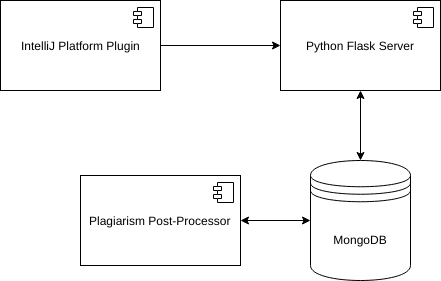
\includegraphics[height=\textheight,
    keepaspectratio=true,
    width=\textwidth,
    ]{figures/architecture-diagram.png}
  }
  \caption[Final design architecture diagram]{Architecture diagram}
  \label{fig:architecture-diagram}
\end{figure}

\vspace*{\fill}

\newpage

\section{Student Plugin Interaction Sequence Diagram}
\autoref{fig:sequence-diagram-student-plugin} shows a typical students' interaction with the plugin. Initially, when a student opens a project, the tracked files are checked for external changes. This is done by comparing each files last known contents (which is stored as a base 64 encoded value) with its current file contents. The difference is added to the list of changes for each file. A DocumentListener is then added to the project for listening to file changes. Each file change is identified and then added to the list of changes for that file. After every new change that is added, the files last known contents is updated (for checking external changes). The recorded data is saved any time a file is saved. File change tracking stops when the project is closed (or if the plugin is disabled or uninstalled).

\vspace*{\fill}

\begin{figure}[H]
  \centering
  \fbox{
    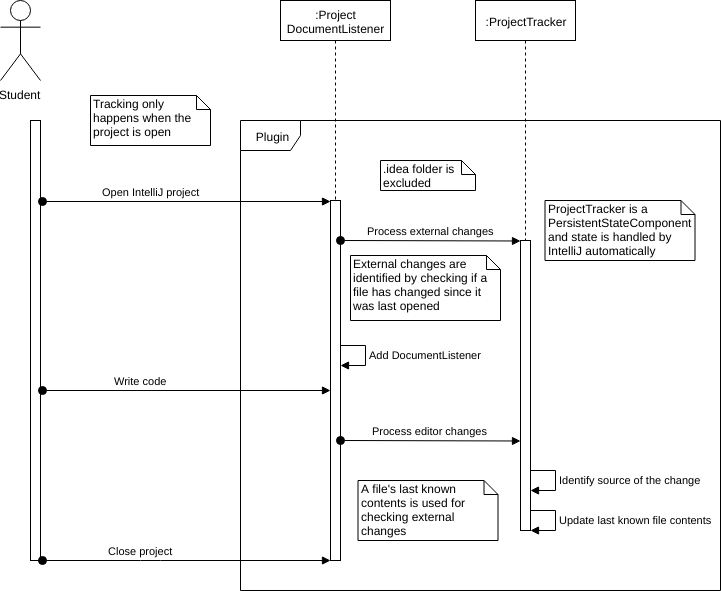
\includegraphics[height=\textheight,
    keepaspectratio=true,
    width=\textwidth,
    ]{figures/sequence-diagram-student-plugin.png}
  }
  \caption[Student-plugin sequence diagram]{Sequence diagram showing a student interacting with the IntelliJ plugin}
  \label{fig:sequence-diagram-student-plugin}
\end{figure}

\vspace*{\fill}

\newpage

\section{Student Server Interaction Sequence Diagram}
\autoref{fig:sequence-diagram-student-server} shows a students' interaction with the server. Once the project is completed. The student may login to the web application using their Aberystwyth University credentials. This authorisation is achieved using the LDAP server provided by Aberystwyth University. This requires the back-end server to be running on the Aberystwyth University network. The LDAP server returns if authentication was successful or not. If successful, then the student will be redirected to their dashboard. A query is sent to the database to retrieve all of the students' submissions. These submissions are then displayed in a table in the dashboard. Students can post new project submissions by uploading the XML file with additional meta data for identification in a form. The form is submitted via POST. The XML file is decrypted and added to the students submissions in the database. The user will be notified of success or failure via a flash message.

\vspace*{\fill}

\begin{figure}[H]
  \centering
  \fbox{
    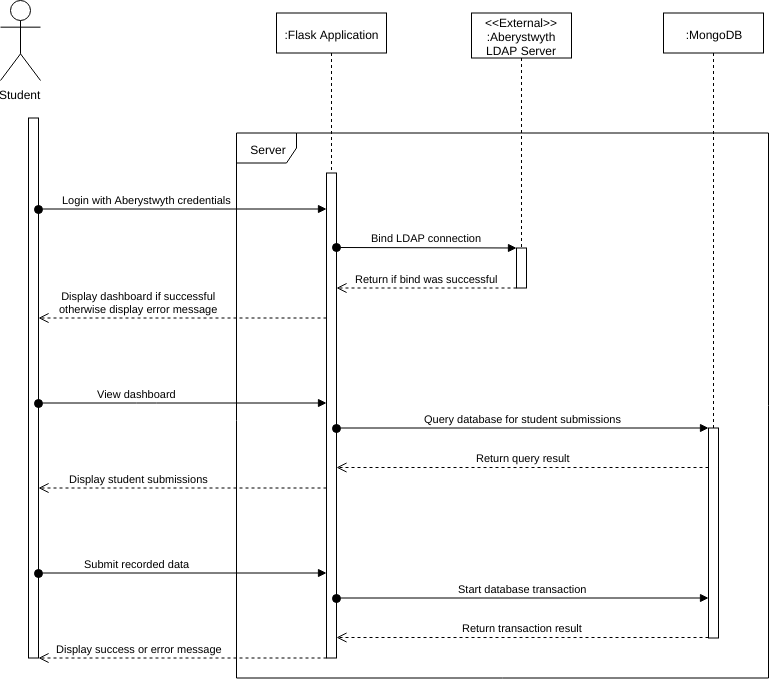
\includegraphics[height=\textheight,
    keepaspectratio=true,
    width=\textwidth,
    ]{figures/sequence-diagram-student-server.png}
  }
  \caption[Student-server sequence diagram]{Sequence diagram showing a student interacting with the server}
  \label{fig:sequence-diagram-student-server}
\end{figure}

\vspace*{\fill}

\newpage

\section{Post-Processor Sequence Diagram}
\autoref{fig:sequence-diagram-post-processor} shows when a student posts a new submission via the web application, the post-processor is notified. This is implemented using the \texttt{watch} method from PyMongo. The \texttt{watch} method notifies the post-processor of all changes in the database in real time. These changes must first be filtered to only identify new submissions. All new submissions are processed and then the resulting data is inserted back into the database using the original submission id and user id. See \autoref{chp:results} for an in-depth review about the post-processor results.

\vspace*{\fill}

\begin{figure}[H]
  \centering
  \fbox{
    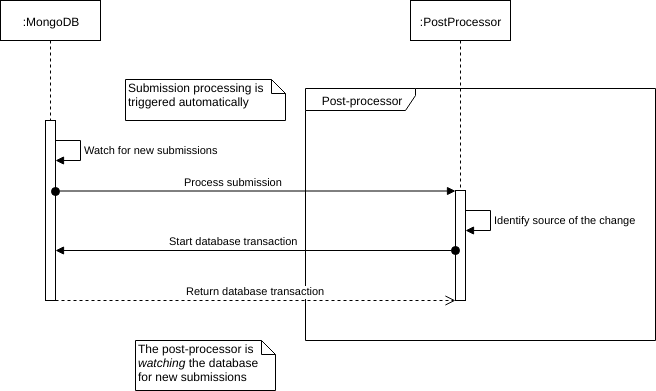
\includegraphics[height=\textheight,
    keepaspectratio=true,
    width=\textwidth,
    ]{figures/sequence-diagram-post-processor.png}
  }
  \caption[Post-processor sequence diagram]{Sequence diagram for the post-processor}
  \label{fig:sequence-diagram-post-processor}
\end{figure}

\vspace*{\fill}

\newpage

\section{Data Structure Class Diagram}
The main class that provides all the tracking is the \texttt{ProjectDocumentListener}. This class detects file changes, refactoring, and external file changes. When changes are detected they are added to the \texttt{ProjectTracker}. The \texttt{ProjectTracker} is used to store all of the changes for a single project. All file changes are stored in a Map data structure. The Map keys are the relative file paths as a String. The Map values are FileTracker objects. The \texttt{ProjectTracker} is also responsible for saving the state of the tracked changes by implementing \texttt{PersistentStateComponent}. An inner class, \texttt{CipherState} is used to store the encrypted Map data. The Map keys are not encrypted but the values are encrypted with 128-bit AES and base64 encoded. \texttt{CipherState} is used to load and save the state. Each tracked file has an associated \texttt{FileTracker} object. This object is used to store each files' Change list and cache. The file cache is its last known contents which is used for detecting external changes. The list of Changes can be used to reconstruct the file and compared with its cache.

\vspace*{\fill}

\begin{figure}[H]
  \centering
  \fbox{
    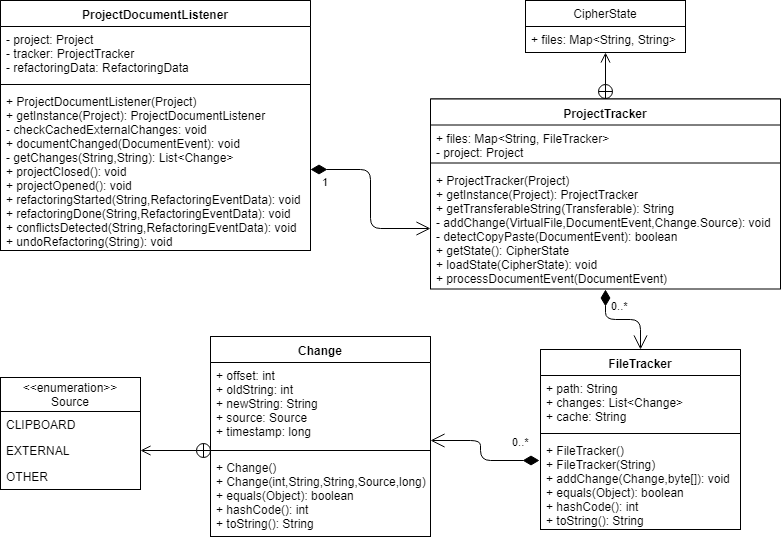
\includegraphics[height=\textheight,
    keepaspectratio=true,
    width=\textwidth,
    ]{figures/plugin-uml-class-diagram.png}
  }
  \caption[Tracked data structure]{Data structure to store tracked data}
  \label{fig:tracked-data-uml-class}
\end{figure}

\vspace*{\fill}

\newpage

\section{Front-end Web Application}
The approach used for designing the front-end web application was based off bootstrap templates. The sign-in page is very simple, containing a simple form to enter credentials.

\begin{figure}[H]
  \centering
  \fbox{
    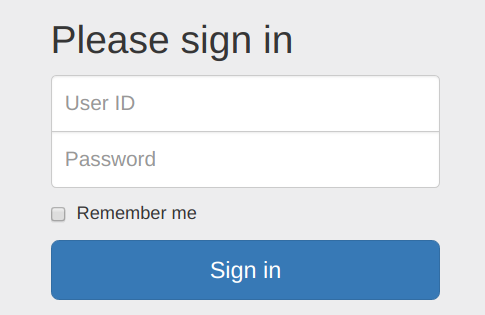
\includegraphics[height=.6\textheight,
    keepaspectratio=true,
    width=.6\textwidth,
    ]{figures/05-web-sign-in.png}
  }
  \caption[Web Sign-in Page]{The index page of the web-application. This is where users sign-in.}
  \label{fig:web-sign-in-page}
\end{figure}

After successful authentication, the user is redirected to the appropriate dashboard. Staff and students have separate dashboards. This is to display different data to each. Students will only see their previous submissions and be able to post new submissions as shown in \autoref{fig:web-student-dashboard}. Staff will be able to view all students submissions and more in-depth details as shown in \autoref{fig:web-staff-dashboard}. The staff submissions table contains three extra columns. The student name, details link, and P value. The student name is to identify the owner of the submission. The details link is to view further details of the submission. The P value is the calculated plagiarism value.

\begin{figure}[H]
  \centering
  \fbox{
    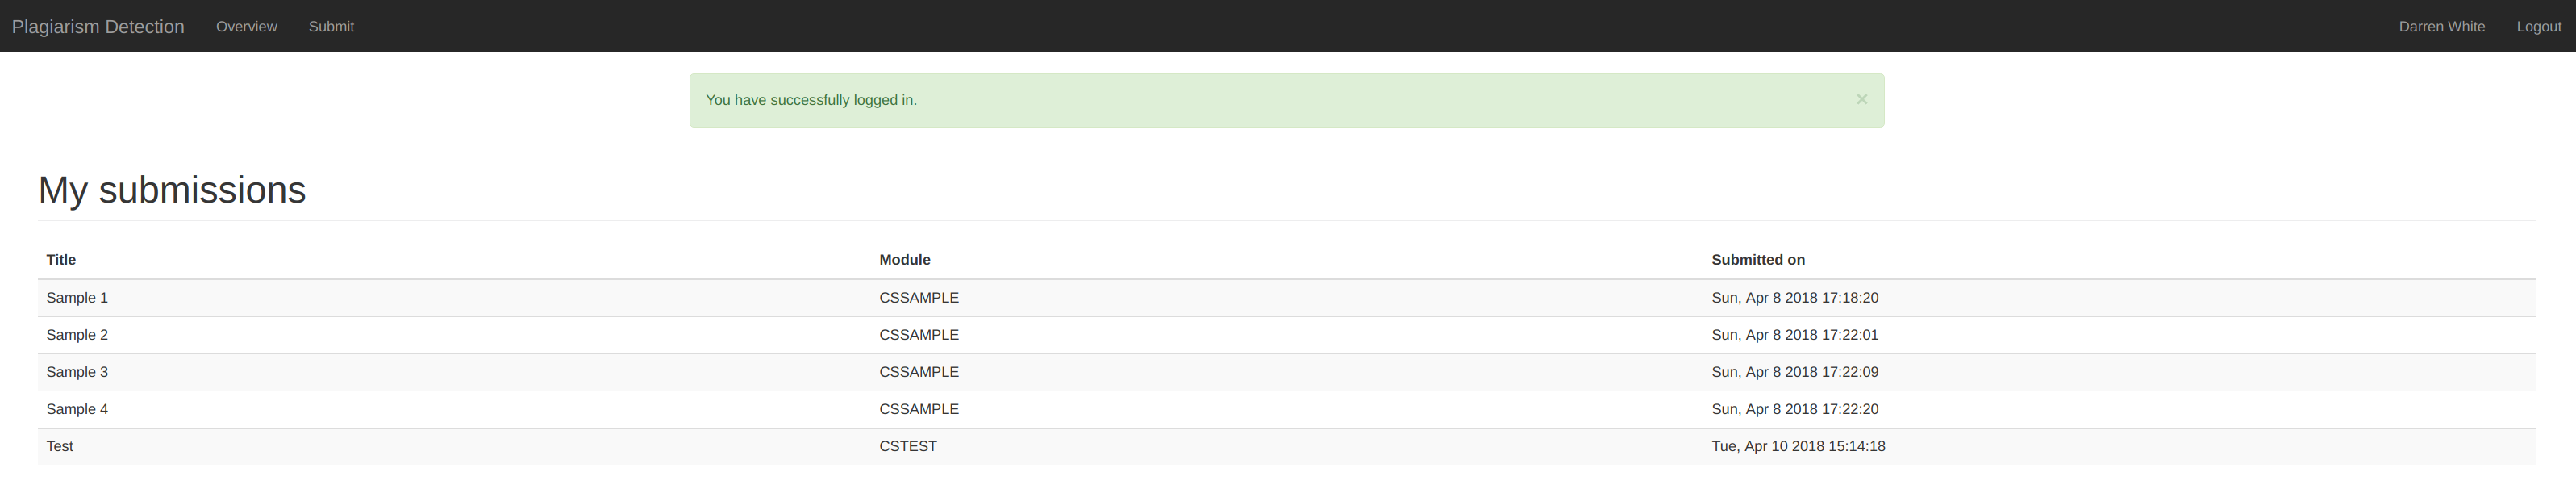
\includegraphics[height=\textheight,
    keepaspectratio=true,
    width=\textwidth,
    ]{figures/07-web-sign-in-success.png}
  }
  \caption[Web Student Dashboard Page]{The dashboard page of the web-application for students.}
  \label{fig:web-student-dashboard}
\end{figure}

\begin{figure}[H]
  \centering
  \fbox{
    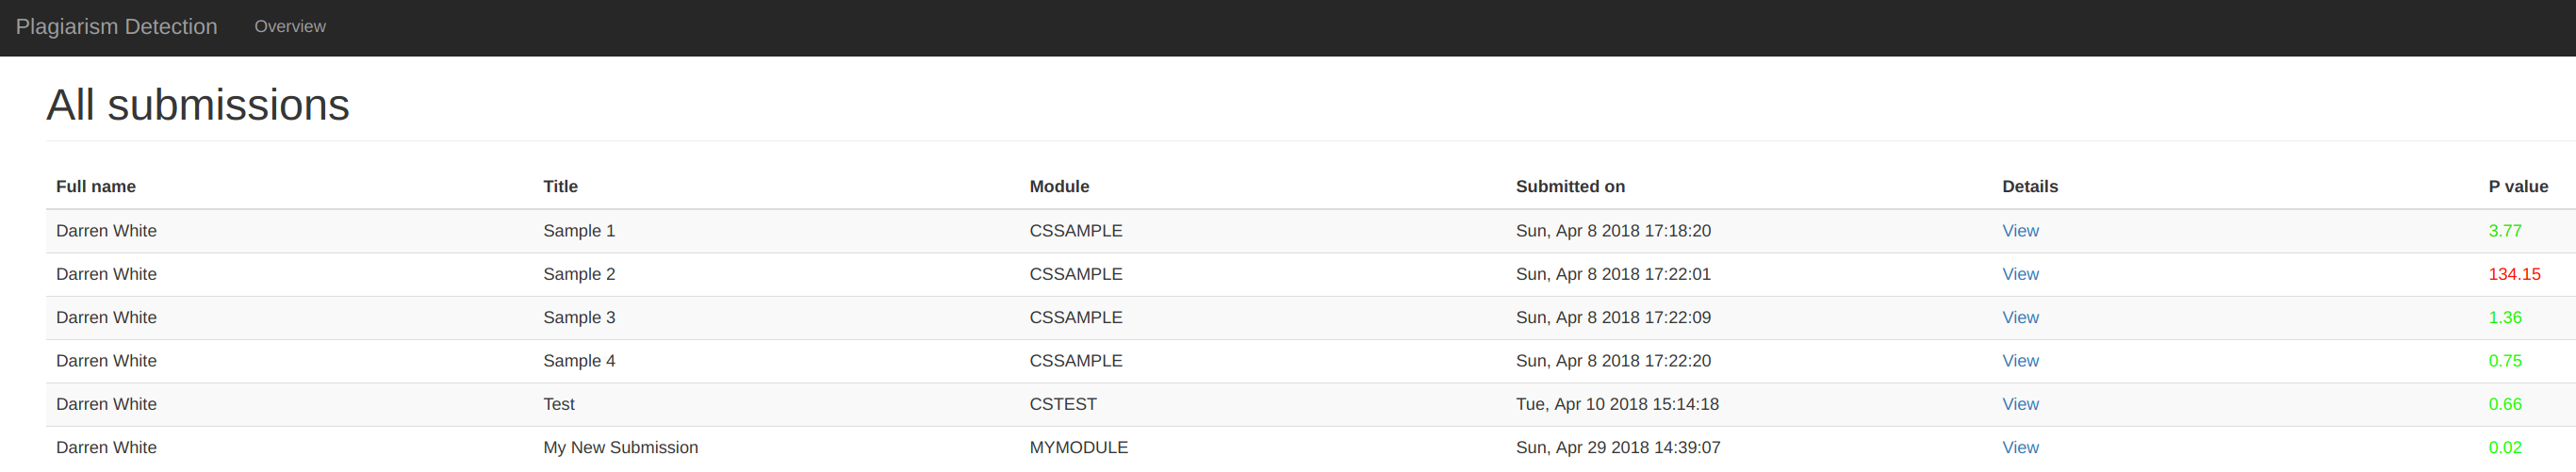
\includegraphics[height=\textheight,
    keepaspectratio=true,
    width=\textwidth,
    ]{figures/10-web-all-submissions.png}
  }
  \caption[Web Staff Dashboard Page]{The dashboard page of the web-application for staff.}
  \label{fig:web-staff-dashboard}
\end{figure}

Staff users are able to view submission details. This includes individual metrics from the post-processor, user and submission details, FTS chart, and large changes. \autoref{fig:web-submission-details-data}, \autoref{fig:web-submission-details-chart}, and \autoref{fig:web-submission-details-changes} show the submission details information displayed on the page. All of this data can be used to help with identifying plagiarism. This is discussed more in-depth in \autoref{chp:results}.

\begin{figure}[H]
  \centering
  \fbox{
    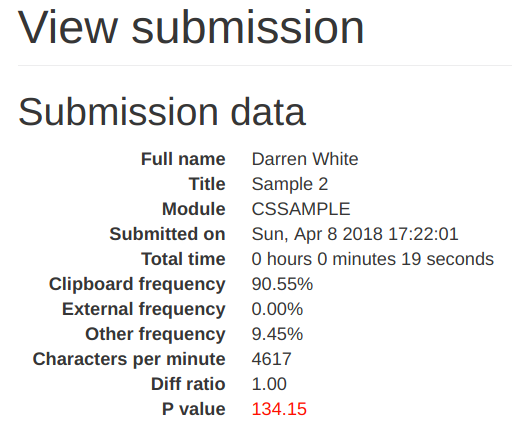
\includegraphics[height=.5\textheight,
    keepaspectratio=true,
    width=.5\textwidth,
    ]{figures/11-web-view-bad-submission-data.png}
  }
  \caption[Web Submission Data]{An example submission metrics view. This shows the submissions post-processed results.}
  \label{fig:web-submission-details-data}
\end{figure}

\begin{figure}[H]
  \centering
  \fbox{
    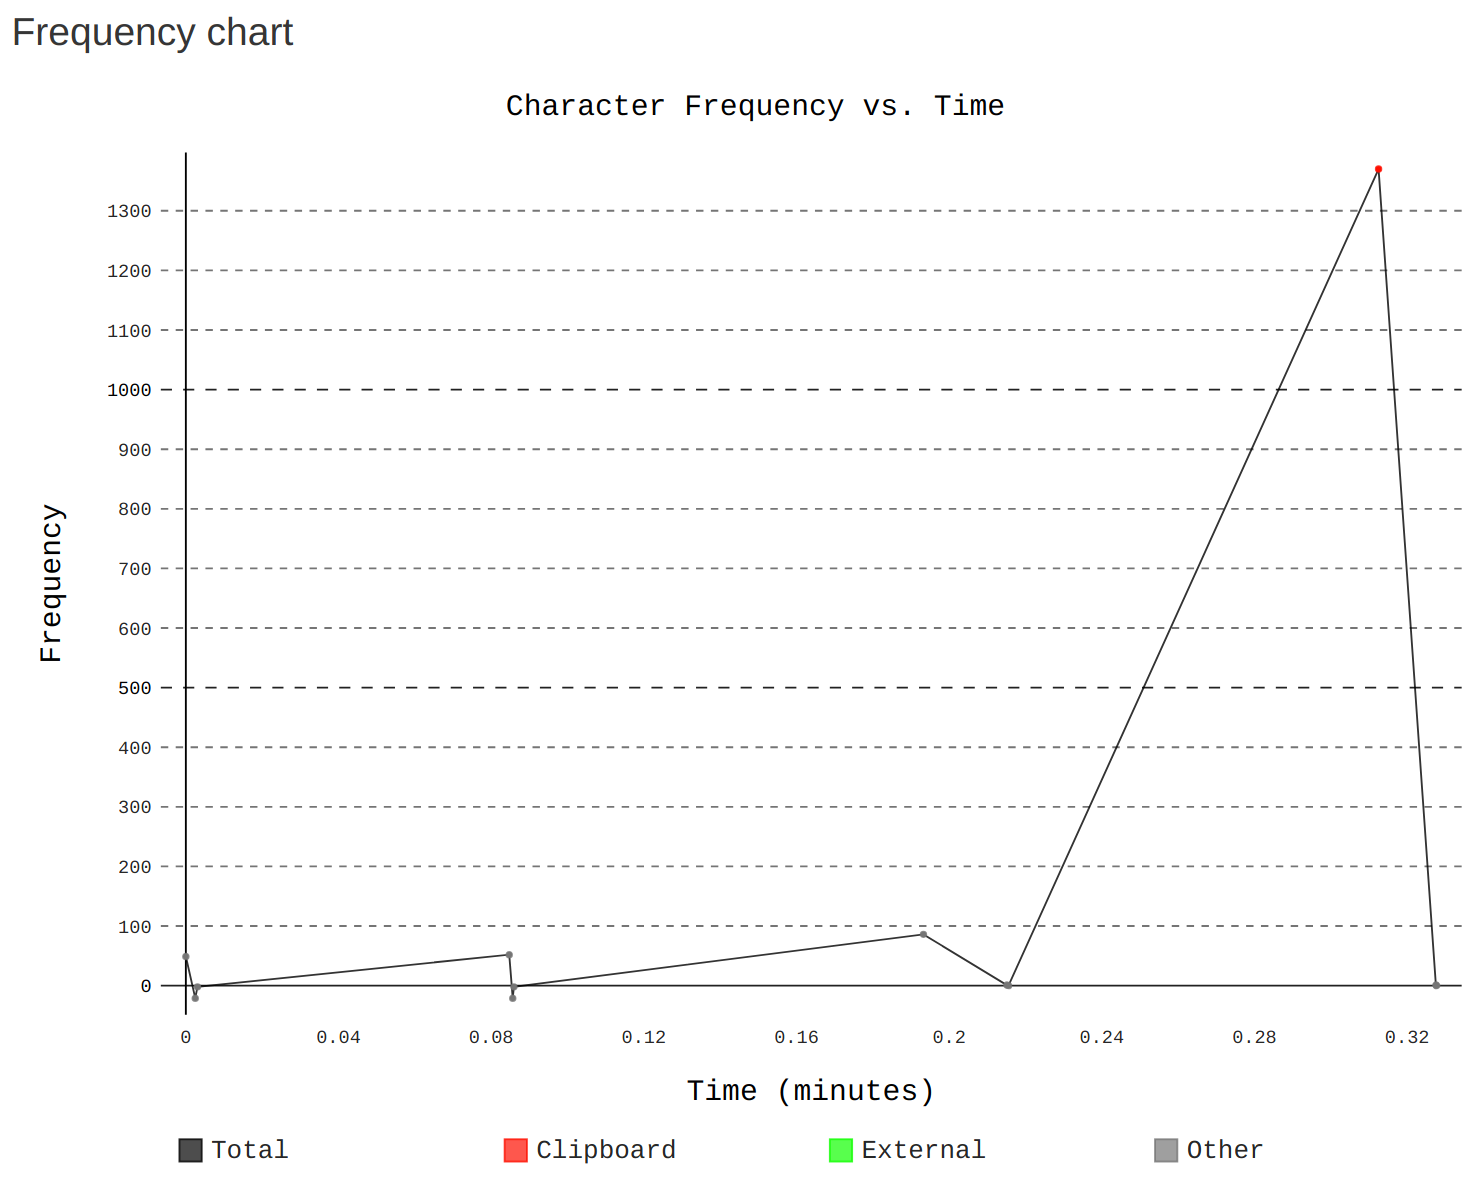
\includegraphics[height=.8\textheight,
    keepaspectratio=true,
    width=.8\textwidth,
    ]{figures/12-web-view-bad-submission-chart.png}
  }
  \caption[Web Submission FTS Chart]{An example submission FTS chart. This shows the type of source code changes over the development time of a submission.}
  \label{fig:web-submission-details-chart}
\end{figure}

\begin{figure}[H]
  \centering
  \fbox{
    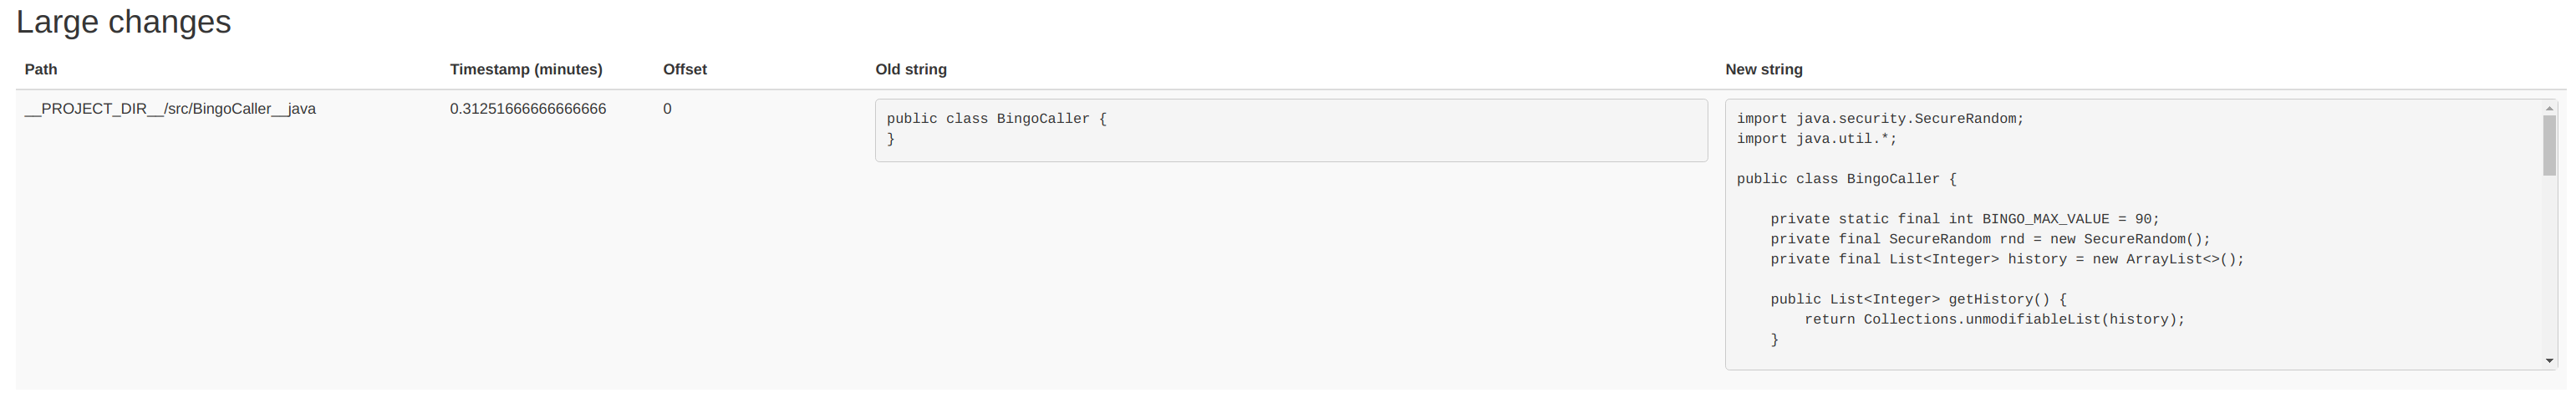
\includegraphics[height=\textheight,
    keepaspectratio=true,
    width=\textwidth,
    ]{figures/13-web-view-bad-submission-changes.png}
  }
  \caption[Web Submission Changes]{An example submission large changes. This shows the major changes tracked for a submission.}
  \label{fig:web-submission-details-changes}
\end{figure}

\newpage

\section{Docker Containers}
The back-end server and post-processor were both written with Docker in mind. Docker containers were used to easily deploy each of the server components. These components are the back-end server, post-processor, and database. Each of these have an individual \texttt{Dockerfile}. Docker Compose is used to seamlessly deploy all of these applications as separate containers with simple commands. See \autoref{cde:docker-compose} for the \texttt{docker-compose.yml} file. The mongodb service is built and deployed as a container first. This is because both the post-processor and server services depend on it. The local \texttt{data/db} directory is mounted to provide persistence for the database across deployments. This allows the container to stop and the data to remain on disk. The post-processor and server past through the \texttt{PDP\_DEBUG} environment variable. This is used by both of the components to enable debug logging when the value is present. The server service mounts the local server directory to the container. This allows Flask to hot-reload when files are changed locally. This removes the need to restart all containers when small changes are made to the server code. Both the mongodb and server services open ports for the containers. This is required for mongodb so that other containers can connect to it. The server opens the port so users can access the web service.

%TC:ignore
\begin{code}
\begin{minted}[breaklines,
               linenos,
               frame=lines]{yaml}
version: '2'
services:
  mongodb:
    build: ./mongodb
    hostname: mongodb
    ports:
      - 27017:27107
    volumes:
      - ./data/db:/data/db
  postprocessor:
    build: ./postprocessor
    depends_on:
      - mongodb
    environment:
      - PDP_DEBUG=${PDP_DEBUG}
  server:
    build: ./server
    depends_on:
      - mongodb
    environment:
      - PDP_DEBUG=${PDP_DEBUG}
    ports:
      - 8000:8000
    volumes:
      - ./server:/plagiarism_detection/server
\end{minted}
\caption{The docker-compose.yml file. This file is used to deploy multiple containers with Docker Compose.}
\label{cde:docker-compose}
\end{code}
%TC:endignore

\autoref{cde:dockerfile-server} shows the Dockerfile for the back-end server. The Dockerfile uses the python base image. This provides the basic Python infrastructure, including the Python interpreter and pip (both version 3). The working directory is configured and system requirements are installed (not pip requirements). The entrypoint script is added. The entrypoint script is executed when the container is created as it is defined as the entrypoint on L22. The requirements file is added and pip is used to install the requirements. L17 is used to add the current local directory to the working directory in the container. This will add the server files to the container. The unit tests are executed using nose. If any tests fail then the container will fail to build and will not run.

%TC:ignore
\begin{code}
\begin{minted}[breaklines,
               linenos,
               frame=lines]{dockerfile}
FROM python:3.6.4-slim

WORKDIR /plagiarism_detection/server

RUN apt-get update && \
    apt-get install -y gcc

ADD entrypoint.sh ./
RUN set -ex && \
    chmod +x entrypoint.sh

ADD requirements.txt ./

RUN set -ex && \
    pip3 install -r requirements.txt

ADD ./ ./

RUN set -ex && \
    nosetests --with-coverage --cover-erase --cover-package=server -v

ENTRYPOINT ["./entrypoint.sh"]
\end{minted}
\caption{The Dockerfile for the server}
\label{cde:dockerfile-server}
\end{code}
%TC:endignore

\autoref{cde:dockerfile-server-entrypoint} shows the entrypoint Bash script for the server as used by the Dockerfile above. This script simply executes the server as a Python module.

%TC:ignore
\begin{code}
\begin{minted}[breaklines,
               linenos,
               frame=lines]{bash}
#!/usr/bin/env bash

SCRIPT_DIR="$( cd "$( dirname "${BASH_SOURCE[0]}" )" && pwd )"

pushd ${SCRIPT_DIR} >/dev/null

python3 -m server
\end{minted}
\caption{The server Dockerfile entrypoint Bash script}
\label{cde:dockerfile-server-entrypoint}
\end{code}
%TC:endignore

\chapter{Testing}
\label{chp:testing}
\section{Strategy}
% Justification for different kinds of test
% What my plan was before I did the testing
The approach used for testing each of the components was limited to unit testing. Having previous experience with unit testing in both Java and Python lead to this decision. The plan for testing the plugin was simple; test each of the detection methods. The plan for testing the server was to test each of the Flask routes to ensure the correct outcome. The post-processor acts as an I/O tool so the plan was to simply test that I/O process. Due to the lack of experience with setting up CI (continuous integration), this was considered but not set up. This would have eased with ensuring breaking changes are not accepted and merged. However, both the server and post-processor will be built as Docker containers and will run the tests as they are built. Any failing tests will fail the build.

\section{Plugin}
JUnit is used for testing the plugin. The IntelliJ Plugin SDK provides a testing infrastructure. This allows testing the plugin in a headless environment. What this means is that the IDE is run without the UI to test all aspects of the plugin. Everything is loaded as usual except the UI. The SDK provides classes and methods to \textit{emulate} user actions such as typing, pasting, clicking menu items, and clicking tool bar buttons. Emulating such actions allows testing of detecting editor changes.

Four classes are included in the tests directory. \texttt{BaseClass} provides useful assertion methods. These will check file changes for specific data. \texttt{CipherTest} is a simple test case for the 128-bit AES encryption on the tracked data. Encrypted and unencrypted sample data is used to test the both the encryption and decryption methods. \texttt{CopyPasteDetectionTest.java} is a core source detection test for detecting copy-paste in the editor. This ensures that all copy-paste actions in the editor are tracked properly. \texttt{ExternalDetectionTest} is another core source detection test for detecting external file changes. This test is a unique test because it needs to simulate externally changing a file without using the IDE editor. This works by notifying the \texttt{ProjectDocumentListener} that the project has closed, making the changes (and therefore making "external" changes), notify the \texttt{ProjectDocumentListener} that the project is opened, which will detect the "external" changes correctly. See the unit test for testing external change detection in \autoref{cde:external-change-test}.

%TC:ignore
\begin{code}
\begin{minted}[breaklines,
               linenos,
               frame=lines]{java}
    public void testExternalChangeDetection() throws IOException {
        ProjectDocumentListener listener =
                ProjectDocumentListener.getInstance(getProject());

        try {
            // Simulate closing the project
            // If we actually close the project then we can't write to the file
            listener.projectClosed();

            // Append the external content
            WriteAction.run(() -> VfsUtil.saveText(file,
                    initialContent + externalContent));
        } finally {
            // Re-open the project
            listener.projectOpened();
        }

        // Check the tracked changes
        assertChangeListSize(filename, 3);
        assertOneChangeMatches(filename, (c) -> c.source == Change.Source.EXTERNAL
                && Objects.equals(c.oldString, "")
                && Objects.equals(c.newString, externalContent)
                && c.offset == 15);
    }
\end{minted}
\caption[External change detection test]{The external change detection unit test. Note that the file is created in the \texttt{setUp()} method with the \texttt{initialContent}}
\label{cde:external-change-test}
\end{code}
%TC:endignore

\section{Server}
Nose is used for testing the back-end server. Nose extends unittest to provide extra functionality. Unittest is built-in to Python 3 and works in a similar manner to JUnit. Mock is a library used to replace parts of the system to change functionality. MockupDB is a library used to mock a MongoDB client.

\texttt{base.py} provides generic \texttt{setUp} and \texttt{tearDown} methods, as well as a method to mock or patch the Aberystwyth LDAP connection. This is useful so that the Aberystwyth LDAP server is not directly contacted but instead is replaced with specific values to return. This removes the need to be connected to the Aberystwyth network when running the unit tests, and any username/password combination may be used for tests. \texttt{test\_data.py} has all necessary testing data for the unit tests.

\texttt{test\_auth.py} contains functions which test the LDAP authentication system. The LDAP connection is patched to provide the necessary user information. The scenarios that are tested are: existing user sign-in, first time user sign-in, invalid user credentials sign-in, checking if user is a staff, and checking if user is a student. See \autoref{cde:first-signin-test} below for the first time sign-in test.

%TC:ignore
\begin{code}
\begin{minted}[breaklines,
               linenos,
               frame=lines]{python}
    @BaseTest.patch_connection(gecos=AberUndergrad.GECOS)
    def test_first_time_signin(self):
        # Send request in background
        future = go(self.app.post, '/', data={
            'uid': AberUndergrad.UID,
            'password': AberUndergrad.PASSWORD,
        })
        # A request is received to check if the user exists
        request = self.mockdb.receives(
            Command('find', 'submissions', filter={'uid': AberUndergrad.UID}))
        # No user exists
        request.ok(cursor={'id': 0, 'firstBatch': [None]})
        # A new User should be inserted
        request = self.mockdb.receives(
            Command('insert', 'submissions'))
        # Request is done
        request.ok()
        # Only one user should be inserted
        documents = request['documents']
        self.assertEqual(1, len(documents))
        # Check the inserted user data
        doc = documents[0]
        self.assertEqual(AberUndergrad.FULL_NAME, doc['full_name'])
        self.assertEqual(AberUndergrad.UID, doc['uid'])
        self.assertEqual(AberUndergrad.USER_TYPE, doc['user_type'])
        self.assertEqual(0, len(doc['submissions']))
        # Check we are redirected to dashboard
        response = future()
        self.assertEqual(response.status_code, 302)
\end{minted}
\caption[Authentication test]{The external change detection unit test. Note that the file is created in the \texttt{setUp()} method with the \texttt{initialContent}. Empty lines have been removed to save space.}
\label{cde:first-signin-test}
\end{code}
%TC:endignore

\texttt{test\_dashboard.py} provides functions to test the staff and student dashboard routes. This involves sending various POST and GET requests to sign-in, and view the dashboard. The various database requests are received and the necessary data is sent as a reply to each request. The dashboard request is checked to ensure adequate data in the submissions table.

\section{Post-Processor}
Nose is also used for testing the post-processor module due to it also being developed with Python 3. MockupDB is also used for mocking the MongoDB client if necessary. The \texttt{base.py} class is very similar to the server \texttt{base.py} file but does not have the function for patching the LDAP connection as this is not used in the post-processor. \texttt{test\_process.py} will test the processing of a submission to ensure the result is as expected. The input is an encrypted XML sample string and the expected output is a dictionary containing the results. The input is processed and the return value is tested. See \autoref{cde:post-processor-test} below for the unit test.

%TC:ignore
\begin{code}
\begin{minted}[breaklines,
               linenos,
               frame=lines]{python}
    def test_process(self):
        # Post process the submission
        result = self.pp.run(StringIO(SUBMISSION_DATA))
        # Check the result
        self.assertEqual(result, SUBMISSION_RESULT)
\end{minted}
\caption[Post-Processor test]{The Post-Processor I/O process unit test.}
\label{cde:post-processor-test}
\end{code}
%TC:endignore

\newpage

\section{Results}
\autoref{fig:tests-plugin}, \autoref{fig:tests-post-processor}, and \autoref{fig:tests-server} show that all of the unit tests for each module pass successfully. \autoref{fig:server-terminal-1} and \autoref{fig:server-terminal-2} show the output from running Docker Compose to deploy the containers.

\begin{figure}[H]
  \centering
  \fbox{
    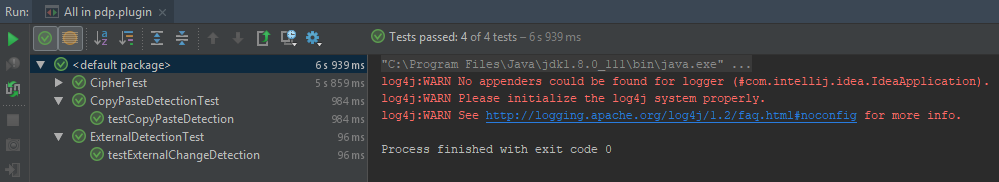
\includegraphics[height=\textheight,
    keepaspectratio=true,
    width=\textwidth,
    ]{figures/00-tests-plugin.png}
  }
  \caption[Plugin tests]{IntelliJ Plugin JUnit tests output}
  \label{fig:tests-plugin}
\end{figure}

\begin{figure}[H]
  \centering
  \fbox{
    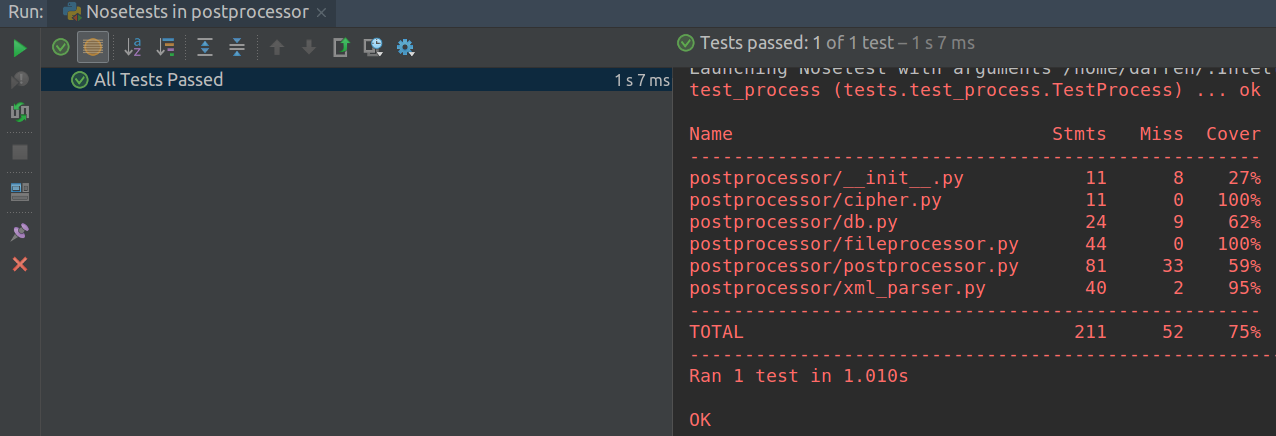
\includegraphics[height=\textheight,
    keepaspectratio=true,
    width=\textwidth,
    ]{figures/01-tests-post-processor.png}
  }
  \caption[Post-processor tests]{Post-processor nose unit tests output}
  \label{fig:tests-post-processor}
\end{figure}

\begin{figure}[H]
  \centering
  \fbox{
    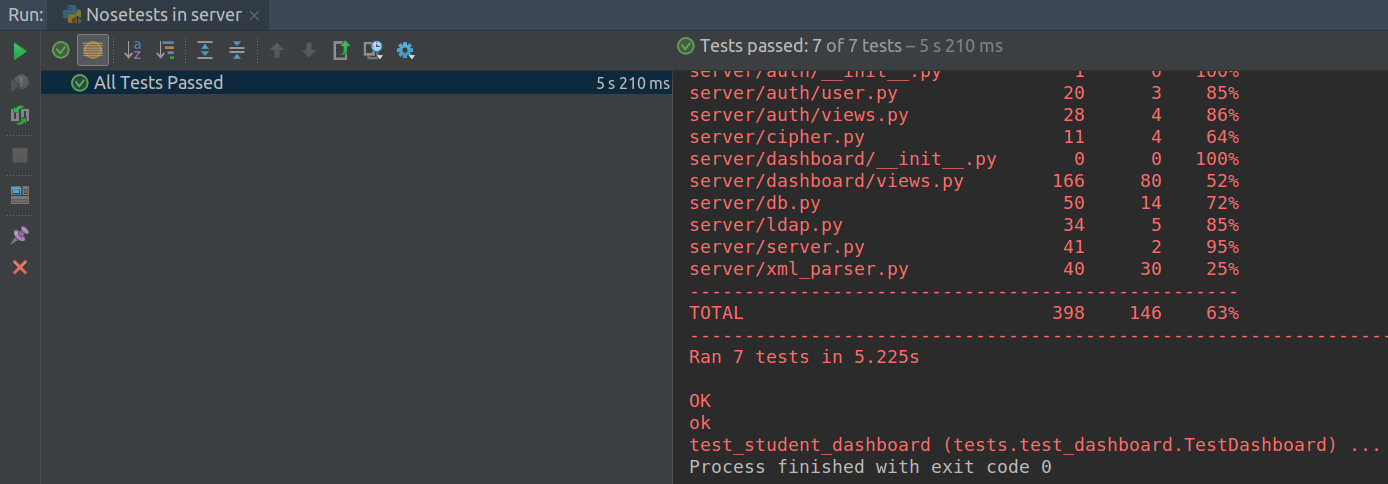
\includegraphics[height=\textheight,
    keepaspectratio=true,
    width=\textwidth,
    ]{figures/02-tests-server.png}
  }
  \caption[Server tests]{Server nose unit tests output}
  \label{fig:tests-server}
\end{figure}

\begin{figure}[H]
  \centering
  \fbox{
    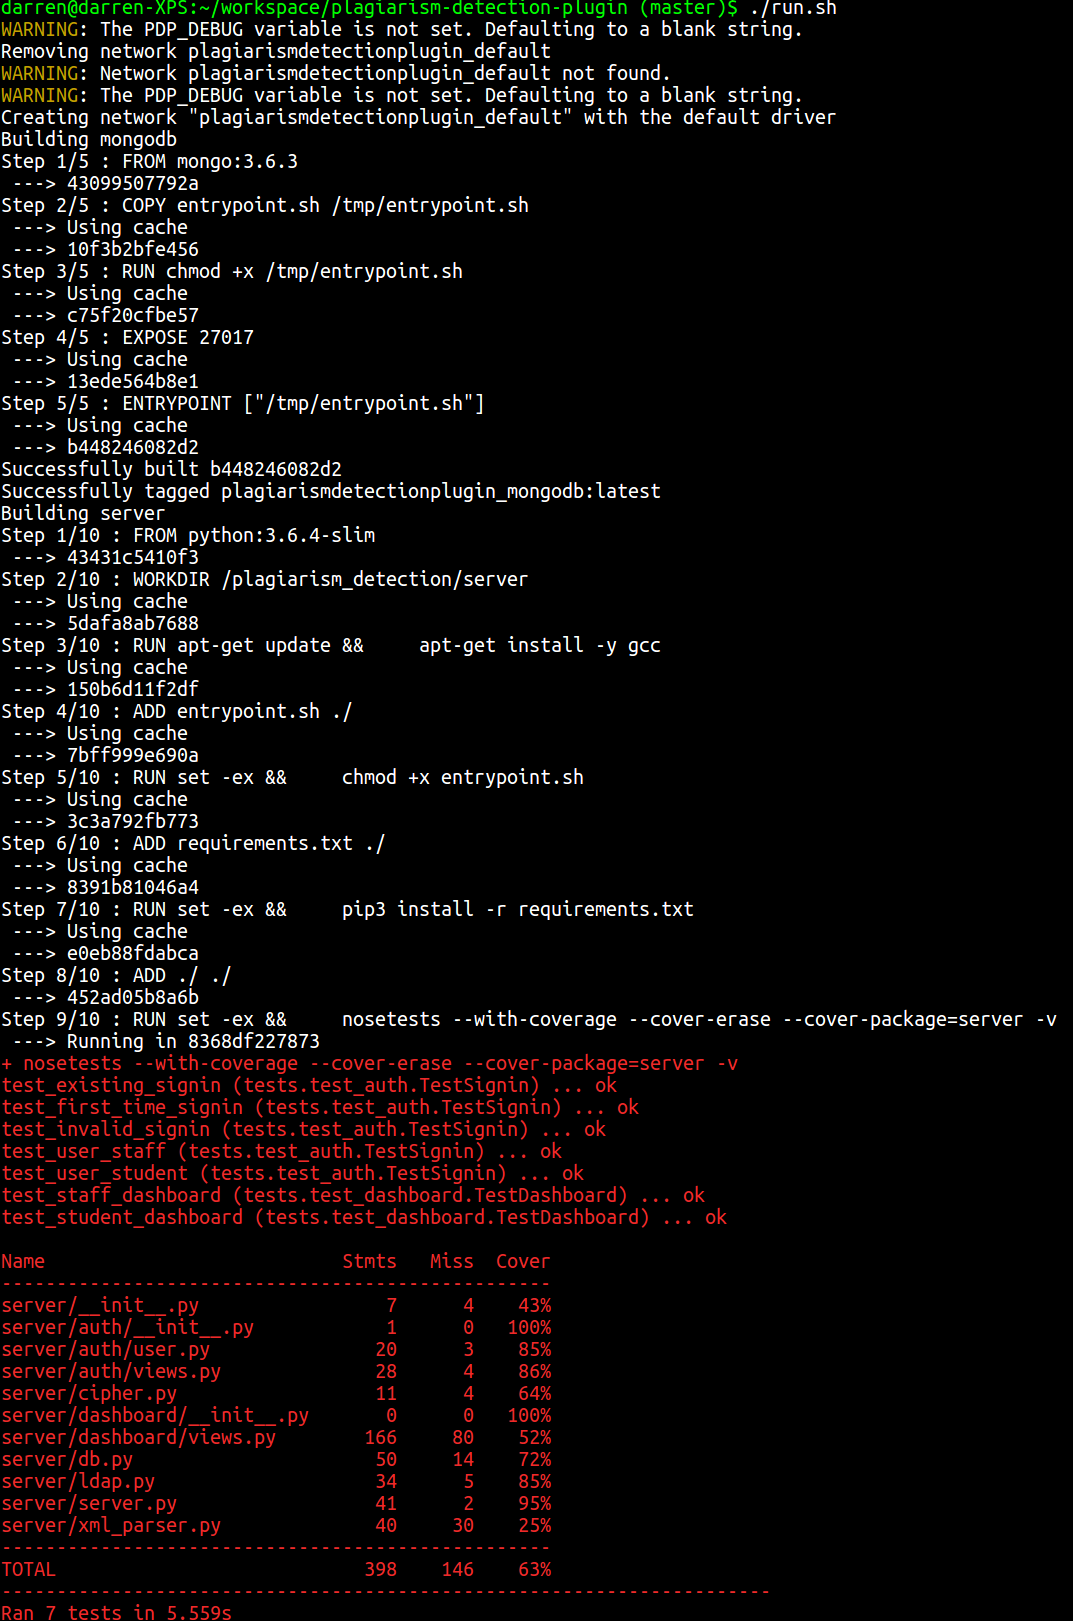
\includegraphics[height=.9\textheight,
    keepaspectratio=true,
    width=.9\textwidth,
    ]{figures/03-server-terminal-1.png}
  }
  \caption[Server Terminal Output 1]{Using Docker Compose to deploy the server. The server and post-processor unit tests are executed in red and all pass successfully.}
  \label{fig:server-terminal-1}
\end{figure}

\begin{figure}[H]
  \centering
  \fbox{
    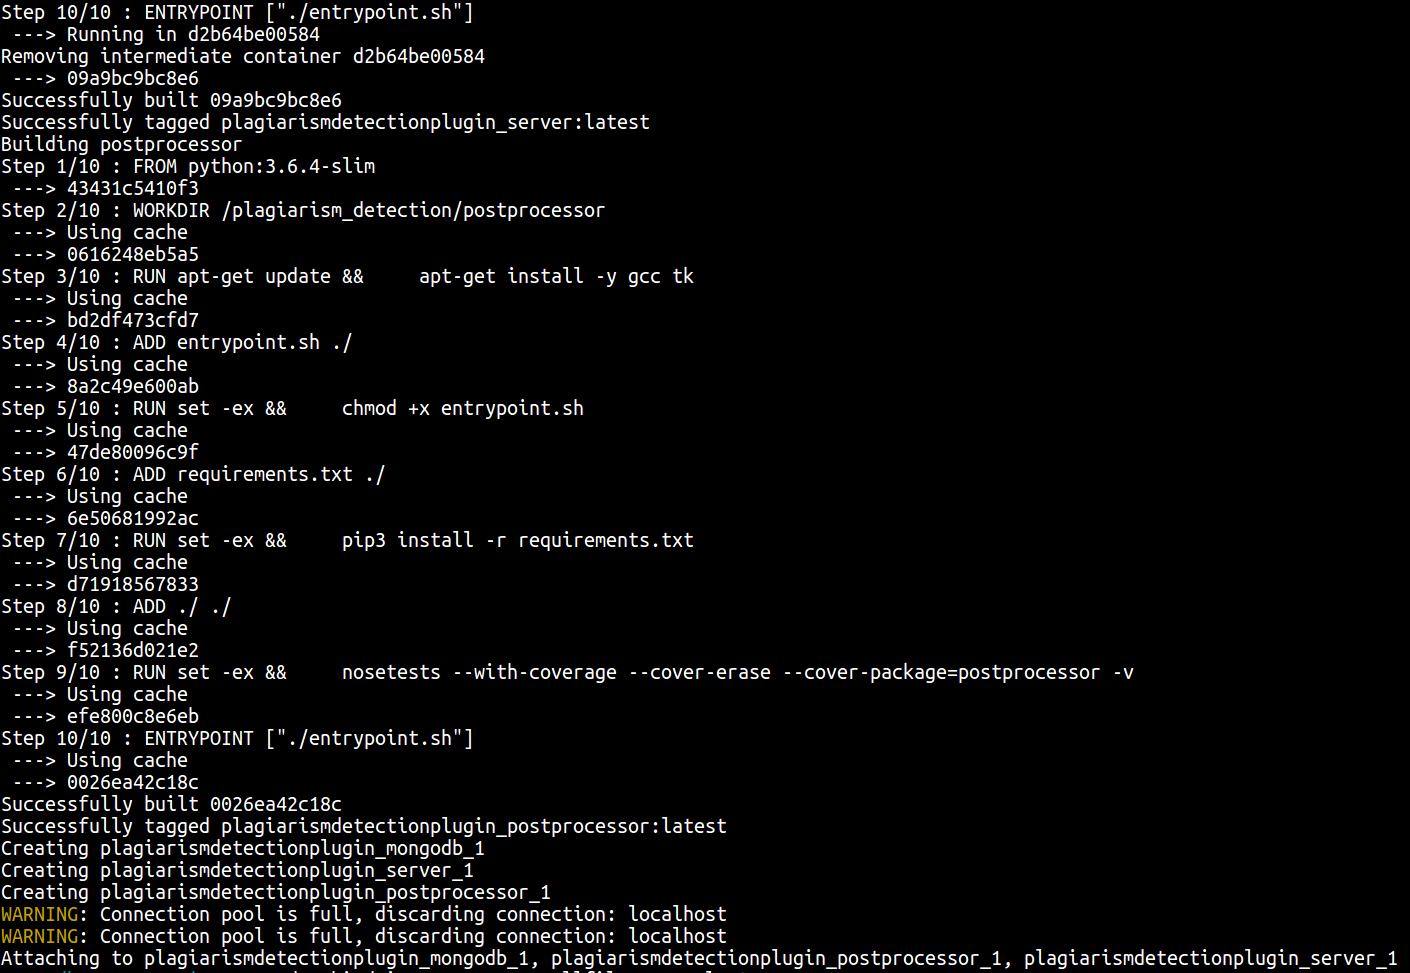
\includegraphics[height=.9\textheight,
    keepaspectratio=true,
    width=.9\textwidth,
    ]{figures/04-server-terminal-2.png}
  }
  \caption[Server Terminal Output 2]{Using Docker Compose to deploy the server. Each of the containers are built successfully and the containers are deployed.}
  \label{fig:server-terminal-2}
\end{figure}



\chapter{Evaluation}
% Examiners expect to find in your dissertation a section addressing such questions as:

% \begin{itemize}
%    \item Were the requirements correctly identified?
%    \item Were the design decisions correct?
%    \item Could a more suitable set of tools have been chosen?
%    \item How well did the software meet the needs of those who were expecting to use it?
%    \item How well were any other project aims achieved?
%    \item If you were starting again, what would you do differently?
% \end{itemize}

% Other questions can be addressed as appropriate for a project.

% Such material is regarded as an important part of the dissertation; it should demonstrate that you are capable not only of carrying out a piece of work but also of thinking critically about how you did it and how you might have done it better. This is seen as an important part of an honours degree.

% There will be good things and room for improvement with any project. As you write this section, identify and discuss the parts of the work that went well and also consider ways in which the work could be improved.

% In the latter stages of the module, we will discuss the evaluation. That will probably be around week 9, although that differs each year.

\chapter{Evaluation}
% Examiners expect to find in your dissertation a section addressing such questions as:

% \begin{itemize}
%    \item Were the requirements correctly identified?
%    \item Were the design decisions correct?
%    \item Could a more suitable set of tools have been chosen?
%    \item How well did the software meet the needs of those who were expecting to use it?
%    \item How well were any other project aims achieved?
%    \item If you were starting again, what would you do differently?
% \end{itemize}

% Other questions can be addressed as appropriate for a project.

% Such material is regarded as an important part of the dissertation; it should demonstrate that you are capable not only of carrying out a piece of work but also of thinking critically about how you did it and how you might have done it better. This is seen as an important part of an honours degree.

% There will be good things and room for improvement with any project. As you write this section, identify and discuss the parts of the work that went well and also consider ways in which the work could be improved.

% In the latter stages of the module, we will discuss the evaluation. That will probably be around week 9, although that differs each year.
The major requirements for this project were an IntelliJ Platform Plugin, back-end server, post-processor, front-end application, and a database. Each of these components were developed up to the point where they operate as intended. The settings GUI for the plugin was not implemented due to the using the continuous server architecture. Code generation, and code auto-completion of the source code detection types were not implemented due to the complexity of the identification process.

The primary design decision between using a continuous or non-continuous server architecture was a huge decision during this project. It impacted the method in which students would interact with the plugin and submit their tracked data. This in turn affected the back-end server internals. This decision was required before fully developing the server. If the continuous design was used then it would have most definitely increased the workload. Testing the direct connection between the plugin and server would be significantly more difficult than being able to individually test each component.

Using MongoDB was a very clear and strong design decision. If a RDBMS was to be used then the tracked data would need to be completely different from its current form. The use of Python has a clear advantage for using MongoDB. The simplicity of using dictionaries lead to simple interactions with the database.

If the project was to be written from scratch again, it would be interesting to have a greater focus on the post-processor. Concentrating more on the identification of possible cases of plagiarism would provide a much better result. The result would be better due to the simplicity of the current identification algorithm being used. Integrating complex algorithms in the post-processor would allow for a more concrete result for each submission.

IntelliJ IDEA offers many ways to interact with the editor. Many were explored during the project including typing, copy and pasting, auto-completion, automatic code generation, and refactoring. Other methods that were not explored were using IdeaVim, and applying Git operations. IdeaVim emulates Vim in the editor. How would the use of this affect the detection methods? Would yank and paste still register as copy and paste? Using Git to stash changes, change branches, or even simply pulling from upstream can all modify files. Would these changes be tracked? If so, would this result in conflicts in the XML file? The XML file would need to be staged in each branch and committed before changing branch. Both IdeaVim, and Git could have been investigated.

\autoref{fig:velocity-chart} shows the velocity for each sprint. The average sprint velocity was 11. \autoref{fig:burndown-chart} shows the burndown for all iterations. Both of these charts show that development started well, slowed in the middle, and gained speed again towards the end. Using the scrum methodology proved successful for developing this project. It allowed, at maximum, a week to be wasted. If a waterfall approach was to be used, a lot more time could have been wasted if problems arose.

\begin{figure}[H]
  \centering
  \fbox{
    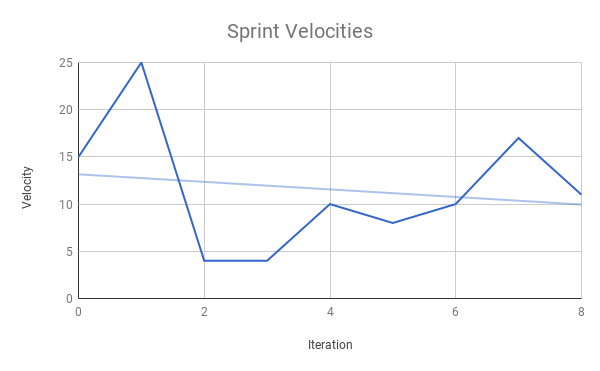
\includegraphics[height=\textheight,
    keepaspectratio=true,
    width=\textwidth,
    ]{figures/velocity-chart.png}
  }
  \caption[Velocity chart]{Velocity for each iteration}
  \label{fig:velocity-chart}
\end{figure}

\begin{figure}[H]
  \centering
  \fbox{
    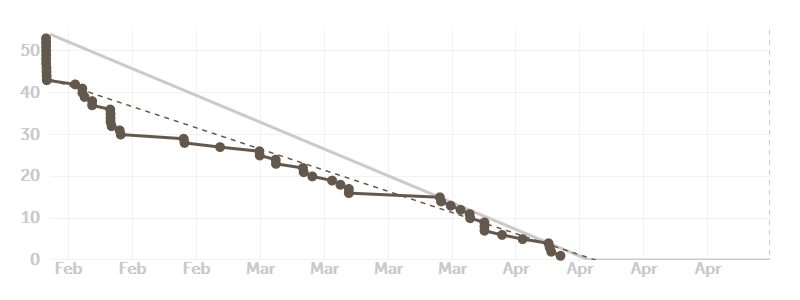
\includegraphics[height=\textheight,
    keepaspectratio=true,
    width=\textwidth,
    ]{figures/burndown-chart.png}
  }
  \caption[Burndown chart]{Burndown chart for all iterations}
  \label{fig:burndown-chart}
\end{figure}


%TC:ignore

\setemptyheader
\addcontentsline{toc}{chapter}{Appendices}
\chapter*{Appendices}

% start the appendix - sets up different numbering
\fancypagestyle{plain}{%
%\fancyhf{} % clear all header and footer fields
\fancyhead[L]{\textsl{Appendix\ \thechapter}}
\fancyhead[R]{\textsl{\leftmark}}}

\appendix
\fancyhead[L]{\textsl{Appendix\ \thechapter}}
\fancyhead[R]{\textsl{\leftmark}}
\fancyhead[C]{}
\fancyfoot[C]{\thepage}
\renewcommand{\headrulewidth}{0.4pt}
\renewcommand{\chaptermark}[1]{\markboth{#1}{}}

\fancyhead[L]{\textsl{Appendix\ \thechapter}}
\fancyhead[R]{\textsl{\leftmark}}
\fancyfoot[C]{{\thepage} of \pageref{LastPage}}

% include any appendices here
\chapter{Third-Party Code and Libraries}
% If you have made use of any third party code or software libraries, i.e. any code that you have not designed and written yourself, then you must include this appendix. 

% As has been said in lectures, it is acceptable and likely that you will make use of third-party code and software libraries. If third party code or libraries are used, your work will build on that to produce notable new work. The key requirement is that we understand what is your original work and what work is based on that of other people. 

% Therefore, you need to clearly state what you have used and where the original material can be found. Also, if you have made any changes to the original versions, you must explain what you have changed. 

% As an example, you might include a definition such as: 

% Apache POI library - The project has been used to read and write Microsoft Excel files (XLS) as part of the interaction with the client's existing system for processing data. Version 3.10-FINAL was used. The library is open source and it is available from the Apache Software Foundation. The library is released using the Apache License. This library was used without modification.

\begin{itemize}
\item \textbf{IntelliJ IDEA 2018.1 and IntelliJ Plugin SDK Build 173.0} - The plugin was developed for the JetBrains IDE, IntelliJ IDEA. This used the open source IntelliJ Plugin SDK. This SDK is released under the Apache License. This library was used without modification.
\item \textbf{JDK 8} - IntelliJ IDEA is built using Java and so the JDK was also used to develop the plugin. The JDK is licensed under the GNU General Public License. This library was used without modification.
\item \textbf{JUnit 4} - JUnit was used to write tests for the plugin. JUnit is released under the Eclipse Public License. This library was used without modification.
\item \textbf{Python 3} - Python 3 was used to write and develop the back-end server and the post-processor. Python 3 is released under the Python Software Foundation License. This library was used without modification.
\item \textbf{Python 3 Packages} - Multiple packages were also used with Python 3:
  \begin{itemize}
  \item \textbf{Coverage v4.5.1} - Coverage was used for unit tests coverage. Coverage is released under the Apache License. This library was used without modification.
  \item \textbf{Flask v0.12.2} - Flask was used to develop the web service for the back-end server. Flask is licensed under a three clause BSD License. This library was used without modification.
  \item \textbf{Flask-Login v0.4.1} - Flask-Login was used to provide authentication services for the back-end server. Flask-Login is licensed under the MIT License. This library was used without modification.
  \item \textbf{ldap3 v2.4.1} - ldap3 was used to provide a connection the an LDAP server for authentication for the back-end server. ldap3 is licensed under the LGPL v3 license. This library was used without modification.
  \item \textbf{Matplotlib v2.2.2} - Matplotlib was used by the post-processor for displaying the FTS charts. Matplotlib uses a license based on the Python Software Foundation License. This library was used without modification.
  \item \textbf{Mock v2.0.0} Mock was used by the post-processor and server to mock parts of the system for unit tests. Mock is licensed under the BSD License. This library was used without modification.
  \item \textbf{MockupDB v1.3.0} - MockupDB was used to mock the MongoDB client for the server and post-processor. MockupDB is licensed under the Apache License. This library was used without modification.
  \item \textbf{Nose v1.3.7} - Nose was used for unit testing the server and post-processor. Nose is licensed under the GNU Lesser General Public License. This library was used without modification.
  \item \textbf{PyCrypto v2.6.1} - PyCrypto was used by the server and post-processor to encrypt and decrypt the XML data. PyCrypto is licensed under Public Domain License. This library was used without modification.
  \item \textbf{Pygal v2.4.0} - Pygal was used to display the FTS chart on the web application. Pygal is licensed under the GNU Lesser General Public License v3. This library was used without modification.
  \item \textbf{PyMongo v3.6.0} - PyMongo was used by the post-processor and server for connecting to the MongoDB server. PyMongo is licensed under the Apache License. This library was used without modification.
  \end{itemize}
\item \textbf{Docker v18.03.0-ce} - Docker was used to build and deploy containers for the server, post-processor, and database. Docker is licensed under the Apache License. This library was used without modification.
\item \textbf{Docker Compose v1.8.0} - Docker Compose was used to deploy the server, post-processor, and database containers together. Docker Compose is licensed under the Apache License. This library was used without modification.
\item \textbf{MongoDB v3.6} - MongoDB was used to store the submitted XML data. MongoDB is licensed under GNU AGPL v3.0. This library was used without modification.
\end{itemize}

\chapter{Ethics Submission}

This appendix includes a copy of the ethics submission for the project. After you have completed your Ethics submission, you will receive a PDF with a summary of the comments. That document should be embedded in this report, either as images, an embedded PDF or as copied text. The content should also include the Ethics Application Number that you receive. 
\chapter{Code Examples}
\label{chp:code-examples}
\section{Example MongoDB Student Document}
\label{sec:mongodb-student-document}

Below is an example MongoDB student document. The document contains the user information retrieved from the Aberystwyth University LDAP server. The submissions array contains all of the students tracked project data. Each submission entry has a one-to-one relation with the XML file. The submission \texttt{\_id} is unique for each submission. The \texttt{\_id} also contains the date which is useful to know when submission was posted. The submission contains input from the student, such as the title and module. The XML file that is submitted is processed and transformed into the correct formatting (JSON) which contains all of the tracked files. Each file has its path, changes, and cache. After post-processing, the result is added to the submission. 

\begin{lstlisting}[
  breaklines = true,
  postbreak  = \mbox{\textcolor{red}{$\hookrightarrow$}\space},
  frame      = single,
  language   = JSON
]
{
  "_id" : ObjectId("5aca40bda326f6001046e1b7"),
  "uid" : "abc12",
  "full_name" : "John Smith",
  "user_type" : "ABUG",
  "submissions" : [
    {
      "_id": ObjectId("5accc6ba7041650010aa3a37"),
      "title": "A Submission",
      "module": "CS12345",
      "files": {
        "src/Test__java": {
          "path": "src/Test.java",
          "changes": [
            {
              "offset": "0",
              "oldString": "",
              "newString": "package PACKAGE_NAME;\n\npublic class Test {\n}\n",
              "source": "OTHER",
              "timestamp": "1522599829159"
            }
          ],
          "cache": "cHVibGljIGNsYXNzIFRlc3QgewoKfQ=="
        }
      },
      "result": {
        "src/Test__java": {
          "diff_ratio": 1,
          "frequency_total": 45,
          "frequency_clipboard": 0,
          "frequency_external": 0,
          "frequency_other": 45,
          "frequency_time_source_data": [
            {
              "f": 45,
              "s": "OTHER",
              "t": NumberLong("1522599829159")
            }
          ]
        }
      }
    }
  ]
}
\end{lstlisting}


\fancypagestyle{plain}{%
   \fancyhead{} %[C]{Annotated Bibliography}
   \fancyfoot[C]{{\thepage} of \pageref{LastPage}} % except the center
   \renewcommand{\headrulewidth}{0pt}
   \renewcommand{\footrulewidth}{0pt}
}

\setemptyheader

\nocite{*} % include everything from the bibliography, irrespective of whether it has been referenced.

% the following line is included so that the bibliography is also shown in the table of contents. There is the possibility that this is added to the previous page for the bibliography. To address this, a newline is added so that it appears on the first page for the bibliography. 
\addcontentsline{toc}{chapter}{Annotated Bibliography} % Adds References to contents page

% example of including an annotated bibliography. The current style is an author date one. If you want to change, comment out the line and uncomment the subsequent line. You should also modify the packages included at the top (see the notes earlier in the file) and then trash your aux files and re-run. 
%\bibliographystyle{authordate2annot}
\bibliographystyle{IEEEannotU}
\renewcommand{\bibname}{Annotated Bibliography} 

\bibliography{references} % References file

%TC:endignore

\end{document}
